% Options for packages loaded elsewhere
\PassOptionsToPackage{unicode}{hyperref}
\PassOptionsToPackage{hyphens}{url}
\PassOptionsToPackage{dvipsnames,svgnames*,x11names*}{xcolor}
%
\documentclass[
  12pt,
]{book}
\usepackage{lmodern}
\usepackage{amssymb,amsmath}
\usepackage{ifxetex,ifluatex}
\ifnum 0\ifxetex 1\fi\ifluatex 1\fi=0 % if pdftex
  \usepackage[T1]{fontenc}
  \usepackage[utf8]{inputenc}
  \usepackage{textcomp} % provide euro and other symbols
\else % if luatex or xetex
  \usepackage{unicode-math}
  \defaultfontfeatures{Scale=MatchLowercase}
  \defaultfontfeatures[\rmfamily]{Ligatures=TeX,Scale=1}
\fi
% Use upquote if available, for straight quotes in verbatim environments
\IfFileExists{upquote.sty}{\usepackage{upquote}}{}
\IfFileExists{microtype.sty}{% use microtype if available
  \usepackage[]{microtype}
  \UseMicrotypeSet[protrusion]{basicmath} % disable protrusion for tt fonts
}{}
\makeatletter
\@ifundefined{KOMAClassName}{% if non-KOMA class
  \IfFileExists{parskip.sty}{%
    \usepackage{parskip}
  }{% else
    \setlength{\parindent}{0pt}
    \setlength{\parskip}{6pt plus 2pt minus 1pt}}
}{% if KOMA class
  \KOMAoptions{parskip=half}}
\makeatother
\usepackage{xcolor}
\IfFileExists{xurl.sty}{\usepackage{xurl}}{} % add URL line breaks if available
\IfFileExists{bookmark.sty}{\usepackage{bookmark}}{\usepackage{hyperref}}
\hypersetup{
  pdftitle={{[}SER 2021 Workshop{]} Causal Mediation: Modern Methods for Path Analysis},
  pdfauthor={Iván Díaz, Nima Hejazi, Kara Rudolph},
  colorlinks=true,
  linkcolor=Maroon,
  filecolor=Maroon,
  citecolor=Blue,
  urlcolor=Blue,
  pdfcreator={LaTeX via pandoc}}
\urlstyle{same} % disable monospaced font for URLs
\usepackage{listings}
\newcommand{\passthrough}[1]{#1}
\lstset{defaultdialect=[5.3]Lua}
\lstset{defaultdialect=[x86masm]Assembler}
\usepackage{longtable,booktabs}
% Correct order of tables after \paragraph or \subparagraph
\usepackage{etoolbox}
\makeatletter
\patchcmd\longtable{\par}{\if@noskipsec\mbox{}\fi\par}{}{}
\makeatother
% Allow footnotes in longtable head/foot
\IfFileExists{footnotehyper.sty}{\usepackage{footnotehyper}}{\usepackage{footnote}}
\makesavenoteenv{longtable}
\usepackage{graphicx,grffile}
\makeatletter
\def\maxwidth{\ifdim\Gin@nat@width>\linewidth\linewidth\else\Gin@nat@width\fi}
\def\maxheight{\ifdim\Gin@nat@height>\textheight\textheight\else\Gin@nat@height\fi}
\makeatother
% Scale images if necessary, so that they will not overflow the page
% margins by default, and it is still possible to overwrite the defaults
% using explicit options in \includegraphics[width, height, ...]{}
\setkeys{Gin}{width=\maxwidth,height=\maxheight,keepaspectratio}
% Set default figure placement to htbp
\makeatletter
\def\fps@figure{htbp}
\makeatother
\setlength{\emergencystretch}{3em} % prevent overfull lines
\providecommand{\tightlist}{%
  \setlength{\itemsep}{0pt}\setlength{\parskip}{0pt}}
\setcounter{secnumdepth}{5}
\usepackage{booktabs}
\usepackage[inline]{enumitem}
\usepackage{float}
\usepackage{graphicx}
\usepackage[round]{natbib}
\usepackage{geometry}
\usepackage{tikz}
\usepackage[english]{babel}
\usepackage{longtable}
\usepackage{color}
\usepackage{mathtools,bm,amssymb,amsmath,amsthm}
\usepackage{multirow}
\usepackage[titletoc,title]{appendix}
\usepackage{authblk}
\usepackage{setspace}
\usepackage{dsfont}
\usepackage[OT1]{fontenc}
\usepackage[bf,singlelinecheck=off]{caption}
\usepackage{refcount}
\usepackage{framed,color}
\definecolor{shadecolor}{RGB}{248,248,248}

\renewcommand{\textfraction}{0.05}
\renewcommand{\topfraction}{0.8}
\renewcommand{\bottomfraction}{0.8}
\renewcommand{\floatpagefraction}{0.75}

%\renewenvironment{quote}{\begin{VF}}{\end{VF}}
\let\oldhref\href
\renewcommand{\href}[2]{#2\footnote{\url{#1}}}

\makeatletter
\newenvironment{kframe}{%
\medskip{}
\setlength{\fboxsep}{.8em}
 \def\at@end@of@kframe{}%
 \ifinner\ifhmode%
  \def\at@end@of@kframe{\end{minipage}}%
  \begin{minipage}{\columnwidth}%
 \fi\fi%
 \def\FrameCommand##1{\hskip\@totalleftmargin \hskip-\fboxsep
 \colorbox{shadecolor}{##1}\hskip-\fboxsep
     % There is no \\@totalrightmargin, so:
     \hskip-\linewidth \hskip-\@totalleftmargin \hskip\columnwidth}%
 \MakeFramed {\advance\hsize-\width
   \@totalleftmargin\z@ \linewidth\hsize
   \@setminipage}}%
 {\par\unskip\endMakeFramed%
 \at@end@of@kframe}
\makeatother

\usepackage{makeidx}
\makeindex

\urlstyle{tt}

\usepackage{amsthm}
\makeatletter
\def\thm@space@setup{%
  \thm@preskip=8pt plus 2pt minus 4pt
  \thm@postskip=\thm@preskip
}
\makeatother

\newtheorem*{remark}{Remark}
\newtheorem{theorem}{Theorem}
\AtEndDocument{\refstepcounter{theorem}\label{finalthm}}
{
  \theoremstyle{definition}
  \newtheorem{assumption}{}
}
{
  \theoremstyle{definition}
  \newtheorem{assumptioniden}{}
}
{
  \theoremstyle{definition}
  \newtheorem{example}{Example}[section]
}
\DeclareMathOperator{\opt}{opt}
\DeclareMathOperator{\dr}{IF}
\newcommand{\hopt}{\hat h_{\opt}}
\newcommand{\supp}{\mathop{\mathrm{supp}}}
\renewcommand\theassumptioniden{{A}\arabic{assumptioniden}}
\renewcommand\theassumption{{C}\arabic{assumption}}
\renewcommand\theexample{\arabic{example}}

\newtheorem{lemma}{Lemma}
\newtheorem{coro}{Corollary}
\newtheorem{definition}{Definition}
\DeclareMathOperator{\expit}{expit}
\DeclareMathOperator{\bern}{Bern}
\DeclareMathOperator{\logit}{logit}
\DeclareMathOperator{\var}{Var}
\DeclareMathOperator{\Rem}{Rem}
\newcommand{\pt}{\mbox{$p_0$}}
\newcommand{\Pt}{\mbox{$P_0$}}
\newcommand{\pl}{\parallel}
\newcommand{\indep}{\mbox{$\perp\!\!\!\perp$}}
\newcommand{\rs}{R}
\newcommand{\ds}{D^\dag}
\newcommand{\dd}{\mathrm{d}}
\newcommand{\Pn}{\mathbb{P}_{n}}
\newcommand{\mut}{\mu_0}
\newcommand{\thetasub}{\hat\theta_{\mbox{\scriptsize sub}}(\delta)}
\newcommand{\thetare}{\hat\theta_{\mbox{\scriptsize re}}(\delta)}
\newcommand{\thetatmle}{\hat\theta_{\mbox{\scriptsize tmle}}(\delta)}
\newcommand{\thetaaipw}{\hat\theta(\delta)}
\newcommand{\hgd}{\hat g_\delta}
\newcommand{\one}{\mathds{1}}
\renewcommand{\P}{\mathbb{P}}
\newcommand{\R}{\mathbb{R}}
\renewcommand{\rmdefault}{ptm}
\newcommand{\I}{\mathbb{I}}
\newcommand{\E}{\mathbb{E}}
\newcommand{\M}{\mathcal{M}}
\newcommand{\1}{\mathbbm{1}}
\newcommand{\prob}{\mathbb{P}}
\renewenvironment{proof}{{\it Proof }}{\qed \\}
\DeclareMathOperator*{\argmin}{\arg\!\min}
\DeclarePairedDelimiterX{\norm}[1]{\lVert}{\rVert}{#1}

% setting bookdown frontmatter option
\frontmatter
\usepackage[]{natbib}
\bibliographystyle{apalike}

\title{{[}SER 2021 Workshop{]} Causal Mediation: Modern Methods for Path Analysis}
\author{Iván Díaz, Nima Hejazi, Kara Rudolph}
\date{updated: May 16, 2021}

\begin{document}
\maketitle

% you may need to leave a few empty pages before the dedication page

%\cleardoublepage\newpage\thispagestyle{empty}\null
%\cleardoublepage\newpage\thispagestyle{empty}\null
%\cleardoublepage\newpage
\thispagestyle{empty}

\begin{center}
%\includegraphics{images/dedication.pdf}
\end{center}

\setlength{\abovedisplayskip}{-5pt}
\setlength{\abovedisplayshortskip}{-5pt}

% setting bookdown mainmatter (e.g., arabic numerals for page numbering)
\mainmatter

{
\hypersetup{linkcolor=}
\setcounter{tocdepth}{2}
\tableofcontents
}
\hypertarget{welcome-to-ser}{%
\chapter*{Welcome to SER!}\label{welcome-to-ser}}


This open source, reproducible vignette accompanies a half-day workshop on
modern methods for \emph{causal mediation analysis}, given at the \href{https://epiresearch.org/annual-meeting/2021-meeting/workshop/}{SER 2021
Meeting} on
Monday, 24 May 2021. While we encourage use of this \passthrough{\lstinline!bookdown!} site, for
convenience, we have also made these workshop materials \href{https://code.nimahejazi.org/ser2021_mediation_workshop/ser2021mediation.pdf}{available in
PDF}.
Discussion will take place \emph{on Slack} -- first join the workspace
\href{https://join.slack.com/t/moderncausalmediation/shared_invite/zt-qd2ocx45-XlKvMA9FXlsixnwI7VnbHQ}{here},
then the ``\#ser2021'' channel.

\hypertarget{about}{%
\section{About this workshop}\label{about}}

Causal mediation analysis can provide a mechanistic understanding of how an
exposure impacts an outcome, a central goal in epidemiology and health sciences.
However, rapid methodologic developments coupled with few formal courses
presents challenges to implementation. Beginning with an overview of classical
direct and indirect effects, this workshop will present recent advances that
overcome limitations of previous methods, allowing for: (i) continuous
exposures, (ii) multiple, non-independent mediators, and (iii) effects
identifiable in the presence of intermediate confounders affected by exposure.
Emphasis will be placed on flexible, stochastic and interventional direct and
indirect effects, highlighting how these may be applied to answer substantive
epidemiological questions from real-world studies. Multiply robust,
nonparametric estimators of these causal effects, and free and open source \passthrough{\lstinline!R!}
packages (\href{https://github.com/nhejazi/medshift}{\passthrough{\lstinline!medshift!}} and
\href{https://github.com/nhejazi/medoutcon}{\passthrough{\lstinline!medoutcon!}}) for their application, will
be introduced.

To ensure translation to real-world data analysis, this workshop will
incorporate hands-on \passthrough{\lstinline!R!} programming exercises to allow participants practice in
implementing the statistical tools presented. It is recommended that
participants have working knowledge of the basic notions of causal inference,
including counterfactuals and identification (linking the causal effect to a
parameter estimable from the observed data distribution). Familiarity with the
\passthrough{\lstinline!R!} programming language is also recommended.

\hypertarget{schedule}{%
\section{Workshop schedule}\label{schedule}}

\begin{itemize}
\tightlist
\item
  10:00A-10:30A: introductions/mediation set up 
\item
  10:30A-11:15A: controlled direct effects, natural direct and indirect effects,
  interventional direct and indirect effects 
\item
  11:15A-11:45A: stochastic mediation estimands 
\item
  11:45A-12:00P: how to choose an estimand in real-world examples 
\item
  12:00P-12:15P break/discussion
\item
  12:15P-12:45P: what is the EIF 
\item
  12:45P-01:00P: using the EIF for estimating the natural direct
  effect 
\item
  01:00P-01:45P: practice: \passthrough{\lstinline!R!} code for estimation 
\item
  01:45P-02:00P: Wrap-up
\end{itemize}

\textbf{NOTE: All times listed in Pacific Time.}

\hypertarget{instructors}{%
\section{About the instructors}\label{instructors}}

\hypertarget{ivuxe1n-duxedaz}{%
\subsection*{Iván Díaz}\label{ivuxe1n-duxedaz}}


I am an Assistant Professor at Weill Cornel Medicine. My research focuses on the
development of non-parametric statistical methods for causal inference from
observational and randomized studies with complex datasets, using machine
learning. This includes but is not limited to mediation analysis, methods for
continuous exposures, longitudinal data including survival analysis, and
efficiency guarantees with covariate adjustment in randomized trials. I am also
interested in general semi-parametric theory, machine learning, and
high-dimensional data.

\hypertarget{nima-hejazi}{%
\subsection*{Nima Hejazi}\label{nima-hejazi}}


I am a PhD candidate in biostatistics at UC Berkeley, working under the joint
direction of Mark van der Laan and Alan Hubbard. My research interests fall at
the intersection of causal inference and machine learning, drawing on ideas from
non/semi-parametric estimation in large, flexible statistical models. Particular
areas of current emphasis include causal mediation analysis, corrections for
outcome-dependent sampling designs, targeted loss-based estimation, and
applications in vaccine efficacy trials. I am also passionate about statistical
computing and open source software development for applied statistics.

\hypertarget{kara-rudolph}{%
\subsection*{Kara Rudolph}\label{kara-rudolph}}


I am an Assistant Professor of Epidemiology at Columbia University. My research
interests are in developing and applying causal inference methods to understand
social and contextual influences on mental health, substance use, and violence
in disadvantaged, urban areas of the United States. My current work focuses on
developing methods for transportability and mediation, and subsequently applying
those methods to understand how aspects of the school and peer environments
mediate relationships between neighborhood factors and adolescent drug use
across populations. More generally, my work on generalizing/ transporting
findings from study samples to target populations and identifying subpopulations
most likely to benefit from interventions contributes to efforts to optimally
target available policy and program resources.

\hypertarget{repro}{%
\section{Reproduciblity}\label{repro}}

These workshop materials were written using \href{http://bookdown.org/}{bookdown},
and the complete source is available on
\href{https://github.com/tlverse/tlverse-handbook}{GitHub}. This version of the book
was built with R version 4.0.5 (2021-03-31), \href{https://pandoc.org/}{pandoc} version \passthrough{\lstinline!r rmarkdown::pandoc\_version()!}, and the following packages:

\begin{longtable}[]{@{}lll@{}}
\toprule
package & version & source\tabularnewline
\midrule
\endhead
bookdown & 0.21.11 & Github (rstudio/bookdown@33c4f70)\tabularnewline
bslib & 0.2.4.9003 & Github (rstudio/bslib@e09af88)\tabularnewline
dagitty & 0.3-1 & CRAN (R 4.0.5)\tabularnewline
data.table & 1.14.0 & CRAN (R 4.0.5)\tabularnewline
downlit & 0.2.1 & CRAN (R 4.0.5)\tabularnewline
dplyr & 1.0.6 & CRAN (R 4.0.5)\tabularnewline
ggdag & 0.2.3 & CRAN (R 4.0.5)\tabularnewline
ggfortify & 0.4.11 & CRAN (R 4.0.5)\tabularnewline
ggplot2 & 3.3.3 & CRAN (R 4.0.5)\tabularnewline
kableExtra & 1.3.4 & CRAN (R 4.0.5)\tabularnewline
knitr & 1.32 & CRAN (R 4.0.5)\tabularnewline
magick & 2.7.1 & CRAN (R 4.0.5)\tabularnewline
medoutcon & 0.1.5 & Github (nhejazi/medoutcon@39820e2)\tabularnewline
medshift & 0.1.4 & Github (nhejazi/medshift@f9e11a9)\tabularnewline
mvtnorm & 1.1-1 & CRAN (R 4.0.5)\tabularnewline
origami & 1.0.3 & CRAN (R 4.0.5)\tabularnewline
pdftools & 2.3.1 & CRAN (R 4.0.5)\tabularnewline
readr & 1.4.0 & CRAN (R 4.0.5)\tabularnewline
rmarkdown & 2.7.11 & Github (rstudio/rmarkdown@e340d75)\tabularnewline
skimr & 2.1.3 & CRAN (R 4.0.5)\tabularnewline
sl3 & 1.4.3 & Github (tlverse/sl3@5cddc6c)\tabularnewline
stringr & 1.4.0 & CRAN (R 4.0.5)\tabularnewline
tibble & 3.1.1 & CRAN (R 4.0.5)\tabularnewline
tidyr & 1.1.3 & CRAN (R 4.0.5)\tabularnewline
\bottomrule
\end{longtable}

\hypertarget{setup}{%
\section{Setup instructions}\label{setup}}

\hypertarget{r-and-rstudio}{%
\subsection{R and RStudio}\label{r-and-rstudio}}

\textbf{R} and \textbf{RStudio} are separate downloads and installations. R is the
underlying statistical computing environment. RStudio is a graphical integrated
development environment (IDE) that makes using R much easier and more
interactive. You need to install R before you install RStudio.

\hypertarget{windows}{%
\subsubsection{Windows}\label{windows}}

\hypertarget{if-you-already-have-r-and-rstudio-installed}{%
\paragraph{If you already have R and RStudio installed}\label{if-you-already-have-r-and-rstudio-installed}}

\begin{itemize}
\tightlist
\item
  Open RStudio, and click on ``Help'' \textgreater{} ``Check for updates''. If a new version is
  available, quit RStudio, and download the latest version for RStudio.
\item
  To check which version of R you are using, start RStudio and the first thing
  that appears in the console indicates the version of R you are
  running. Alternatively, you can type \passthrough{\lstinline!sessionInfo()!}, which will also display
  which version of R you are running. Go on the \href{https://cran.r-project.org/bin/windows/base/}{CRAN
  website} and check whether a
  more recent version is available. If so, please download and install it. You
  can \href{https://cran.r-project.org/bin/windows/base/rw-FAQ.html\#How-do-I-UNinstall-R_003f}{check here}
  for more information on how to remove old versions from your system if you
  wish to do so.
\end{itemize}

\hypertarget{if-you-dont-have-r-and-rstudio-installed}{%
\paragraph{If you don't have R and RStudio installed}\label{if-you-dont-have-r-and-rstudio-installed}}

\begin{itemize}
\tightlist
\item
  Download R from
  the \href{http://cran.r-project.org/bin/windows/base/release.htm}{CRAN website}.
\item
  Run the \passthrough{\lstinline!.exe!} file that was just downloaded
\item
  Go to the \href{https://www.rstudio.com/products/rstudio/download/\#download}{RStudio download
  page}
\item
  Under \emph{Installers} select \textbf{RStudio x.yy.zzz - Windows
  XP/Vista/7/8} (where x, y, and z represent version numbers)
\item
  Double click the file to install it
\item
  Once it's installed, open RStudio to make sure it works and you don't get any
  error messages.
\end{itemize}

\hypertarget{macos-mac-os-x}{%
\subsubsection{macOS / Mac OS X}\label{macos-mac-os-x}}

\hypertarget{if-you-already-have-r-and-rstudio-installed-1}{%
\paragraph{If you already have R and RStudio installed}\label{if-you-already-have-r-and-rstudio-installed-1}}

\begin{itemize}
\tightlist
\item
  Open RStudio, and click on ``Help'' \textgreater{} ``Check for updates''. If a new version is
  available, quit RStudio, and download the latest version for RStudio.
\item
  To check the version of R you are using, start RStudio and the first thing
  that appears on the terminal indicates the version of R you are running.
  Alternatively, you can type \passthrough{\lstinline!sessionInfo()!}, which will also display which
  version of R you are running. Go on the \href{https://cran.r-project.org/bin/macosx/}{CRAN
  website} and check whether a more
  recent version is available. If so, please download and install it.
\end{itemize}

\hypertarget{if-you-dont-have-r-and-rstudio-installed-1}{%
\paragraph{If you don't have R and RStudio installed}\label{if-you-dont-have-r-and-rstudio-installed-1}}

\begin{itemize}
\tightlist
\item
  Download R from
  the \href{http://cran.r-project.org/bin/macosx}{CRAN website}.
\item
  Select the \passthrough{\lstinline!.pkg!} file for the latest R version
\item
  Double click on the downloaded file to install R
\item
  It is also a good idea to install \href{https://www.xquartz.org/}{XQuartz} (needed
  by some packages)
\item
  Go to the \href{https://www.rstudio.com/products/rstudio/download/\#download}{RStudio download
  page}
\item
  Under \emph{Installers} select \textbf{RStudio x.yy.zzz - Mac OS X 10.6+ (64-bit)}
  (where x, y, and z represent version numbers)
\item
  Double click the file to install RStudio
\item
  Once it's installed, open RStudio to make sure it works and you don't get any
  error messages.
\end{itemize}

\hypertarget{linux}{%
\subsubsection{Linux}\label{linux}}

\begin{itemize}
\tightlist
\item
  Follow the instructions for your distribution
  from \href{https://cloud.r-project.org/bin/linux}{CRAN}, they provide information
  to get the most recent version of R for common distributions. For most
  distributions, you could use your package manager (e.g., for Debian/Ubuntu run
  \passthrough{\lstinline!sudo apt-get install r-base!}, and for Fedora \passthrough{\lstinline!sudo yum install R!}), but we
  don't recommend this approach as the versions provided by this are
  usually out of date. In any case, make sure you have at least R 3.3.1.
\item
  Go to the \href{https://www.rstudio.com/products/rstudio/download/\#download}{RStudio download
  page}
\item
  Under \emph{Installers} select the version that matches your distribution, and
  install it with your preferred method (e.g., with Debian/Ubuntu \passthrough{\lstinline!sudo dpkg -i rstudio-x.yy.zzz-amd64.deb!} at the terminal).
\item
  Once it's installed, open RStudio to make sure it works and you don't get any
  error messages.
\end{itemize}

These setup instructions are adapted from those written for \href{http://www.datacarpentry.org/R-ecology-lesson/}{Data Carpentry: R
for Data Analysis and Visualization of Ecological
Data}.

\hypertarget{mediation}{%
\chapter{Preliminaries on causal mediation analysis}\label{mediation}}

\hypertarget{motivating-study}{%
\section{Motivating study}\label{motivating-study}}

Do differences in the effects of treatment (comparing two medications for opioid use disorder, naltrexone vs buprenorphine) on risk of relapse operate through mediators of adherence, opioid use, pain, and depressive symptoms? \citep{rudolph2020explaining}

\begin{figure}

{\centering 
\includegraphics[width=0.5\linewidth]{/home/runner/work/ser2021_mediation_workshop/ser2021_mediation_workshop/img/ctndag} 

}

\end{figure}

\hypertarget{what-is-causal-mediation-analysis}{%
\section{What is causal mediation analysis?}\label{what-is-causal-mediation-analysis}}

\begin{itemize}
\tightlist
\item
  Causal mediation analyses assess how the paths behave under interventions
\item
  Statistical mediation analyses assess associations between the variables
\end{itemize}

\hypertarget{why-are-the-methods-that-we-will-discuss-today-important}{%
\subsection{Why are the methods that we will discuss today important?}\label{why-are-the-methods-that-we-will-discuss-today-important}}

\begin{itemize}
\tightlist
\item
  Assume you are interested in the effect of a treatment assignment \(A\) (naltrexone vs.
  buprenorphine) on an outcome \(Y\) (risk of relapse) through mediators \(M\)
  (opioid use, pain, depressive symptoms)
\item
  We have pre-treatment confounders \(W\)
\item
  There is a confounder \(Z\) of \(M\rightarrow Y\) ffected by treatment assignment (adherence)
\item
  We could fit the following models:
  \begin{align}
      \E(M\mid A=a, W=w, Z=z) & = \gamma_0 + \gamma_1 a + \gamma_2 w + \gamma_3 z \\
      \E(Y\mid M=m, A=a, W=w, Z=z) & = \beta_0 + \beta_1 m + \beta_2 a + \beta_3 w + \beta_4 z
    \end{align}
\item
  The product \((\gamma_1\beta_1)\) has been proposed as a measure of the effect
  of \(A\) on \(Y\) through \(M\)
\item
  Causal interpretation problems with this method:

  \begin{itemize}
  \tightlist
  \item
    We will see that this parameter cannot be interpreted as a causal effect
  \end{itemize}
\end{itemize}

\hypertarget{r-example}{%
\subsection{\texorpdfstring{\texttt{R} Example:}{R Example:}}\label{r-example}}

\begin{itemize}
\tightlist
\item
  Assume we have a pre-treamtment confounder of \(Y\) and \(M\), denote it with \(W\)
\item
  For simplicity, assume \(A\) is randomized
\item
  We'll generate a really large sample from a data generating mechanism so that
  we are not concerned with sampling errors
\end{itemize}

\begin{lstlisting}[language=R]
n <- 1e6
w <- rnorm(n)
a <- rbinom(n, 1, 0.5)
z <- rbinom(n, 1, 0.2 * a + 0.3)
m <- rnorm(n, w + z)
y <- rnorm(n, m + w - a + z)
\end{lstlisting}

\begin{itemize}
\tightlist
\item
  Note that the indirect effect (i.e., the effect through \(M\)) in this example
  is nonzero (there is a pathway \(A\rightarrow Z \rightarrow M \rightarrow Y\))
\item
  Let's see what the product of coefficients method would say:
\end{itemize}

\begin{lstlisting}[language=R]
lm_y <- lm(y ~ m + a + w + z)
lm_m <- lm(m ~ a + w + z)
## product of coefficients
coef(lm_y)[2] * coef(lm_m)[2]
#>          m 
#> -0.0014835
\end{lstlisting}

Among other things, in this workshop:

\begin{itemize}
\tightlist
\item
  We will provide some understanding for why the above method fails in this example
\item
  We will study estimators that are robust to misspecification in the above models
\end{itemize}

\hypertarget{causal-mediation-models}{%
\section{Causal mediation models}\label{causal-mediation-models}}

In this workshop we will use directed acyclic graphs. We will focus on the two
types of graph:

\hypertarget{no-intermediate-confounders}{%
\subsection{No intermediate confounders}\label{no-intermediate-confounders}}

\begin{figure}

{\centering \includegraphics[width=0.8\linewidth]{01-preface_files/figure-latex/unnamed-chunk-4-1} 

}

\caption{Directed acyclic graph under *no intermediate confounders* of the mediator-outcome relation affected by treatment}\label{fig:unnamed-chunk-4}
\end{figure}

\hypertarget{intermediate-confounders}{%
\subsection{Intermediate confounders}\label{intermediate-confounders}}

\begin{figure}

{\centering \includegraphics[width=0.8\linewidth]{01-preface_files/figure-latex/unnamed-chunk-5-1} 

}

\caption{Directed acyclic graph under intermediate confounders of the mediator-outcome relation affected by treatment}\label{fig:unnamed-chunk-5}
\end{figure}

The above graphs can be interpreted as a \emph{non-parametric structural equation model}
(NPSEM), also known as \emph{structural causal model} (SCM):

\begin{align}
  W & = f_W(U_W)\\
  A & = f_A(W, U_A)\\
  Z & = f_Z(W, A, U_Z)\\
  M & = f_M(W, A, Z, U_M)\\
  Y & = f_Y(W, A, Z, M, U_Y)
\end{align}

\begin{itemize}
\tightlist
\item
  Here \(U=(U_W, U_A, U_Z, U_M, U_Y)\) is a vector of all unmeasured exogenous
  factors affecting the system
\item
  The functions \(f\) are assumed fixed but unknown
\item
  We posit this model as a system of equations that nature uses to geenrate the
  data
\item
  Therefore we leave the functions \(f\) unspecified (i.e., we do not know the
  true nature mechanisms)
\item
  Sometimes we know something: e.g., if \(A\) is randomized we know \(A=f_A(U_A)\)
  where \(U_A\) is the flip of a coin (i.e., independent of everything).
\end{itemize}

\hypertarget{counterfactuals}{%
\section{Counterfactuals}\label{counterfactuals}}

\begin{itemize}
\tightlist
\item
  We define all the effects of interest using \emph{counterfactuals}
\item
  Counterfactuals are hypothetical random variables that would have been
  observed in an alternative world where something had happened, possibly
  contrary to fact 
\item
  \(Y_a\) is a counterfactual variable in a hypothetical world where \(\P(A=a)=1\)
  with probability one
\item
  \(Y_{a,m}\) is the counterfactual outcome in a world where \(\P(A=a,M=m)=1\)
\item
  \(M_a\) is the counterfactual variable representing the mediator in a world
  where \(\P(A=a)=1\).
\end{itemize}

\hypertarget{how-are-counterfactuals-defined}{%
\subsection{How are counterfactuals defined?}\label{how-are-counterfactuals-defined}}

\begin{itemize}
\tightlist
\item
  In the NPSEM framework, counterfactuals are quantities \emph{derived} from the
  model.
\item
  Take as example the DAG in Figure 1.2:
  \begin{align}
    Y_a  &= f_Y(W, a, Z_a, M_a, U_Y)\\
    Y_{a,m}  &= f_Y(W, a, Z_a, m, U_Y)\\
    M_a  &= f_M(W, a, Z_a, U_M)
  \end{align}
\item
  You can also define \emph{nested counterfactuals}
\item
  For example, if \(A\) is binary, you can think of the following counterfactual
  \begin{equation*}
    Y_{1, M_0} = f_Y(W, 1, Z_1, M_0, U_Y)
  \end{equation*}
\item
  Interpreted as \emph{the outcome for an individual in a hypothetical world where
  treatment was given but the mediator was held at the value it would have
  taken under no treatment}
\item
  Causal effects are defined in terms of the distribution of these
  counterfactuals.
\item
  That is, causal effects give you information about what would have happened
  \emph{in some hypothetical world}.
\end{itemize}

\hypertarget{estimands}{%
\chapter{Path-specific casual mediation effect types}\label{estimands}}

\begin{itemize}
\tightlist
\item
  Controlled direct effects
\item
  Natural direct and indirect effects
\item
  Interventional direct and indirect effects
\end{itemize}

\begin{figure}

{\centering \includegraphics[width=0.8\linewidth]{02-effects-def_files/figure-latex/unnamed-chunk-1-1} 

}

\caption{Directed acyclic graph under *no intermediate confounders* of the mediator-outcome relation affected by treatment}\label{fig:unnamed-chunk-1}
\end{figure}

\hypertarget{controlled-direct-effects}{%
\section{Controlled direct effects}\label{controlled-direct-effects}}

\begin{itemize}
\tightlist
\item
  Set the mediator to a reference value \(M=m\) uniformly for everyone in the
  population
\item
  Compare \(A=1\) vs \(A=0\) with \(M=m\) fixed
\end{itemize}

\[\psi_{\text{CDE}} = \E(Y_{1,m} - Y_{0,m}) \]

\begin{figure}

{\centering 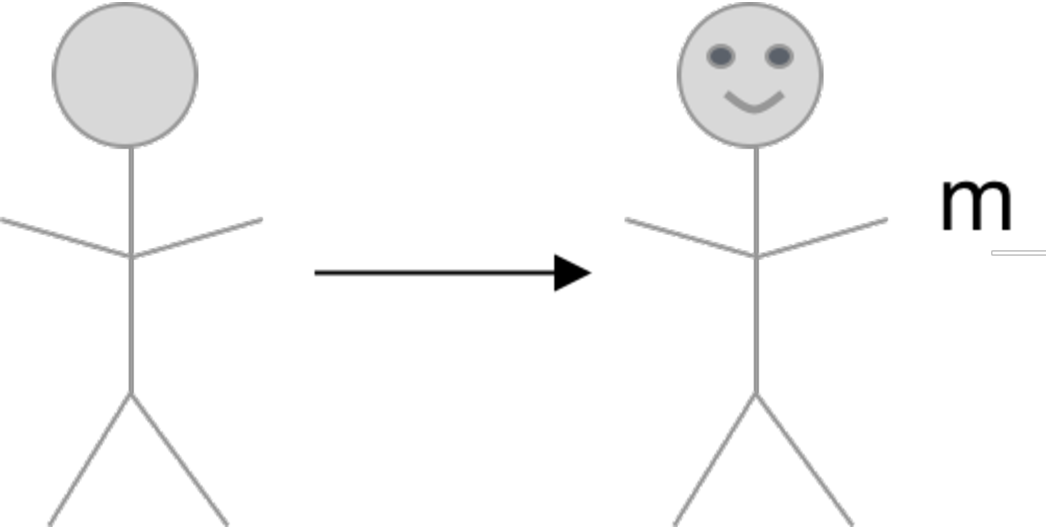
\includegraphics[width=0.5\linewidth]{/home/runner/work/ser2021_mediation_workshop/ser2021_mediation_workshop/img/graphic4a3} 

}

\end{figure}

\hypertarget{identification-assumptions}{%
\subsection{Identification assumptions:}\label{identification-assumptions}}

\begin{itemize}
\tightlist
\item
  Confounder assumptions:

  \begin{itemize}
  \tightlist
  \item
    \(A \indep Y_{a,m} \mid W\)
  \item
    \(M \indep Y_{a,m} \mid W, A\)
  \end{itemize}
\item
  Positivity assumptions:

  \begin{itemize}
  \tightlist
  \item
    \(\P(M = m \mid A=a, W) > 0 \text{  } a.e.\)
  \item
    \(\P(A=a \mid W) > 0 \text{  } a.e.\)
  \end{itemize}
\end{itemize}

Under the above identification assumptions, the controlled direct effect can be
identified:
\[ \E(Y_{1,m} - Y_{0,m}) = \E\{\color{ForestGreen}{\E(Y \mid A=1, M=m, W) - \E(Y \mid A=0, M=m, W)}\}\]

\begin{itemize}
\tightlist
\item
  For intuition about this formula in R, let's continue with a toy example:
\end{itemize}

\begin{lstlisting}[language=R]
n <- 1e6
w <- rnorm(n)
a <- rbinom(n, 1, 0.5)
m <- rnorm(n, w + a)
y <- rnorm(n, w + a + m)
\end{lstlisting}

\begin{itemize}
\tightlist
\item
  First we fit a correct model for the outcome
\end{itemize}

\begin{lstlisting}[language=R]
lm_y <- lm(y ~ m + a + w)
\end{lstlisting}

\begin{itemize}
\tightlist
\item
  Assume we would like the CDE at \(m=0\)
\item
  Then we generate predictions \[\color{ForestGreen}{\E(Y \mid A=1, M=m, W)}
  \text{ and }\color{ForestGreen}{\E(Y \mid A=0, M=m, W)}:\]
\end{itemize}

\begin{lstlisting}[language=R]
pred_y1 <- predict(lm_y, newdata = data.frame(a = 1, m = 0, w = w))
pred_y0 <- predict(lm_y, newdata = data.frame(a = 0, m = 0, w = w))
\end{lstlisting}

\begin{itemize}
\tightlist
\item
  Then we compute the difference between the predicted values
  \(\color{ForestGreen}{\E(Y \mid A=1, M=m, W) - \E(Y \mid A=0, M=m, W)}\), and
  average across values of \(W\)
\end{itemize}

\begin{lstlisting}[language=R]
## CDE at m = 0
mean(pred_y1 - pred_y0)
#> [1] 1.0009
\end{lstlisting}

\hypertarget{is-this-the-estimand-i-want}{%
\subsection{Is this the estimand I want?}\label{is-this-the-estimand-i-want}}

\begin{itemize}
\tightlist
\item
  Makes the most sense if can intervene directly on \(M\)

  \begin{itemize}
  \tightlist
  \item
    And can think of a policy that would set everyone to a single constant
    level \(m \in \mathcal{M}\).
  \item
    J. Pearl calls this \emph{prescriptive}.
  \item
    Can you think of an example?
  \item
    Air pollution, rescue inhaler dosage, hospital visits
  \item
    Does not provide a decomposition of the average treatment effect into
    direct and indirect effects
  \end{itemize}
\end{itemize}

\emph{What if our research question doesn't involve intervening directly on the
mediator?}

\emph{What if we want to decompose the average treatment effect into its direct and
indirect counterparts?}

\hypertarget{natural-direct-and-indirect-effects}{%
\section{Natural direct and indirect effects}\label{natural-direct-and-indirect-effects}}

Still using the same DAG as above,

\begin{itemize}
\tightlist
\item
  Recall the definition of the nested counterfactual
\end{itemize}

\begin{equation*}
    Y_{1, M_0} = f_Y(W, 1, Z_1, M_0, U_Y)
\end{equation*}

\begin{itemize}
\item
  Interpreted as \emph{the outcome for an individual in a hypothetical world where
  treatment was given but the mediator was held at the value it would have
  taken under no treatment}

  \begin{figure}

  {\centering 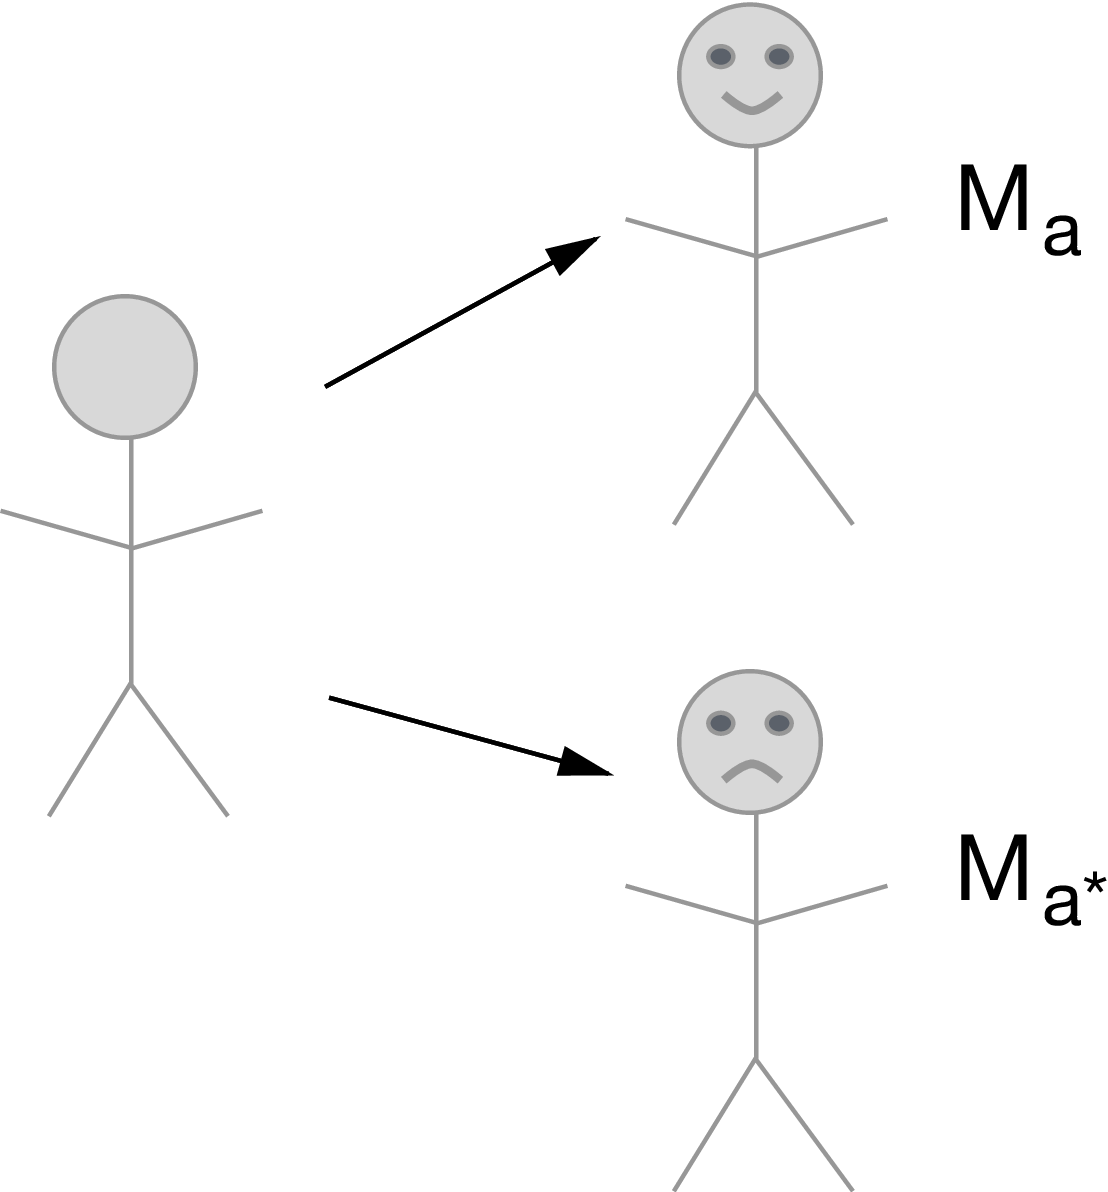
\includegraphics[width=0.5\linewidth]{/home/runner/work/ser2021_mediation_workshop/ser2021_mediation_workshop/img/graphic4a} 

  }

  \end{figure}
\item
  Recall that, because of the definition of counterfactuals
  \begin{equation*}
  Y_{1, M_1} = Y_1
  \end{equation*}
\end{itemize}

Then we can decompose the \emph{average treatment effect} \(E(Y_1-Y_0)\) as follows

\begin{equation*}
\E[Y_{1,M_1} - Y_{0,M_0}] = \underbrace{\E[Y_{\color{red}{1},\color{blue}{M_1}} -
    Y_{\color{red}{1},\color{blue}{M_0}}]}_{\text{natural indirect effect}} +
    \underbrace{\E[Y_{\color{blue}{1},\color{red}{M_0}} -
    Y_{\color{blue}{0},\color{red}{M_0}}]}_{\text{natural direct effect}}
\end{equation*}

\begin{itemize}
\tightlist
\item
  Natural direct effect (NDE): Varying treatment while keeping the mediator
  fixed at the value it would have taken under no treatment
\item
  Natural indirect effect (NIE): Varying the mediator from the value it would
  have taken under treatment to the value it would have taken under control,
  while keeping treatment fixed
\end{itemize}

\hypertarget{identification-assumptions-1}{%
\subsection{Identification assumptions:}\label{identification-assumptions-1}}

\begin{itemize}
\tightlist
\item
  \(A \indep Y_{a,m} \mid W\)
\item
  \(M \indep Y_{a,m} \mid W, A\)
\item
  \(A \indep M_a \mid W\)
\item
  \(M_0 \indep Y_{1,m} \mid W\)
\item
  and positivity assumptions
\end{itemize}

\hypertarget{cross-world-independence-assumption}{%
\subsection{Cross-world independence assumption}\label{cross-world-independence-assumption}}

What does \(M_0 \indep Y_{1,m} \mid W\) mean?

\begin{itemize}
\tightlist
\item
  Conditional on \(W\), knowledge of the mediator value in the absence of
  treatment, \(M_0\),
  provides no information about the outcome under treatment, \(Y_{1,m}\).
\item
  Can you think of a data-generating mechanism that would violate this
  assumption?
\item
  Example: in a randomized study, whenever we believe that treatment assignment
  works through adherence (i.e., almost
  always), we are violating this assumption (more on this later).
\item
  Cross-world assumptions are problematic for other reasons, including:

  \begin{itemize}
  \tightlist
  \item
    You can never design a randomized study where the assumption holds by
    design.
  \end{itemize}
\end{itemize}

\textbf{If the cross-world assumption holds, can write the NDE as a weighted average
of controlled direct effects at each level of \(M=m\).}

\[\E \sum_m \{\E(Y_{1,m} \mid W) - \E(Y_{0,m} \mid W)\} \P(M_{0}=m
\mid W)\]

\begin{itemize}
\tightlist
\item
  If CDE(\(m\)) is constant across \(m\), then CDE = NDE.
\end{itemize}

\hypertarget{identification-formula}{%
\subsection{Identification formula:}\label{identification-formula}}

\begin{itemize}
\item
  Under the above identification assumptions, the natural direct effect can be
  identified:
  \begin{equation*}
  \E(Y_{1,M_0} - Y_{0,M_0}) =
  \E[\color{Goldenrod}{\E\{}\color{ForestGreen}{\E(Y \mid A=1, M, W) -
  \E(Y \mid A=0, M, W)}\color{Goldenrod}{\mid A=0,W\}}]
  \end{equation*}
\item
  The natural indirect effect can be identified similarly.
\item
  Let's dissect this formula in \passthrough{\lstinline!R!}:
\end{itemize}

\begin{lstlisting}[language=R]
n <- 1e6
w <- rnorm(n)
a <- rbinom(n, 1, 0.5)
m <- rnorm(n, w + a)
y <- rnorm(n, w + a + m)
\end{lstlisting}

\begin{itemize}
\tightlist
\item
  First we fit a correct model for the outcome
\end{itemize}

\begin{lstlisting}[language=R]
lm_y <- lm(y ~ m + a + w)
\end{lstlisting}

\begin{itemize}
\tightlist
\item
  Then we generate predictions \[\color{ForestGreen}{\E(Y \mid A=1, M, W)}
  \text{ and }\color{ForestGreen}{\E(Y \mid A=0, M, W)}\] with \(A\) fixed but
  letting \(M\) and \(W\) take their observed
  values
\end{itemize}

\begin{lstlisting}[language=R]
pred_y1 <- predict(lm_y, newdata = data.frame(a = 1, m = m, w = w))
pred_y0 <- predict(lm_y, newdata = data.frame(a = 0, m = m, w = w))
\end{lstlisting}

\begin{itemize}
\tightlist
\item
  Then we compute the difference between the predicted values
  \[\color{ForestGreen}{\E(Y \mid A=1, M, W) - \E(Y \mid A=0, M, W)},\]
\item
  and use this difference as a pseudo-outcome in a regression on \(A\) and \(W\):
  \[\color{Goldenrod}{\E\{}\color{ForestGreen}{\E(Y \mid A=1, M, W) - \E(Y \mid
  A=0, M, W)}\color{Goldenrod}{\mid A=0,W\}}\]
\end{itemize}

\begin{lstlisting}[language=R]
pseudo <- pred_y1 - pred_y0
lm_pseudo <- lm(pseudo ~ a + w)
\end{lstlisting}

\begin{itemize}
\tightlist
\item
  Now we predict the value of this pseudo-outcome under \(A=0\), and average the
  result
\end{itemize}

\begin{lstlisting}[language=R]
pred_pseudo <- predict(lm_pseudo, newdata = data.frame(a = 0, w = w))
## NDE:
mean(pred_pseudo)
#> [1] 0.99655
\end{lstlisting}

\hypertarget{is-this-the-estimand-i-want-1}{%
\subsection{Is this the estimand I want?}\label{is-this-the-estimand-i-want-1}}

\begin{itemize}
\tightlist
\item
  Makes sense to intervene on \(A\) but not directly on \(M\).
\item
  Want to understand a natural mechanism underlying an association/ total
  effect. J. Pearl calls this \emph{descriptive}.
\item
  NDE + NIE = total effect (ATE).
\item
  Okay with the assumptions.
\end{itemize}

\emph{What if our data structure involves a post-treatment confounder of the
mediator-outcome relationship (e.g., adherence)?}

\begin{figure}

{\centering \includegraphics[width=0.8\linewidth]{02-effects-def_files/figure-latex/unnamed-chunk-12-1} 

}

\caption{Directed acyclic graph under intermediate confounders of the mediator-outcome relation affected by treatment}\label{fig:unnamed-chunk-12}
\end{figure}

\begin{figure}

{\centering 
\includegraphics[width=1\linewidth]{/home/runner/work/ser2021_mediation_workshop/ser2021_mediation_workshop/img/ctndag} 

}

\end{figure}

\hypertarget{unidentifiability-of-the-nde-and-nie-in-this-setting}{%
\subsection{Unidentifiability of the NDE and NIE in this setting}\label{unidentifiability-of-the-nde-and-nie-in-this-setting}}

\begin{itemize}
\tightlist
\item
  In this example, natural direct and indirect effects are unidentifiable from observed data \(O=(W,A,Z,M,Y)\).
\item
  The reason for this is that the cross-world counterfactual
  assumption
  \begin{equation*}
  Y_{1,m}\indep M_0\mid W
  \end{equation*}
  does not hold in the above directed acyclic graph.
\item
  Technically, the reason for this is that an intervention setting \(A=1\)
  (necessary for the definition of \(Y_{1,m}\)) induces a counterfactual variable
  \(Z_1\).
\item
  Likewise, an intervention setting \(A=0\) (necessary for the definition of
  \(M_0\)) induces a counterfactual \(Z_0\).
\item
  The variables \(Z_1\) and \(Z_0\) are correlated because they share unmeasured
  common causes, \(U_Z\).
\item
  The variable \(Z_1\) is correlated with \(Y_{1,m}\), and the variable \(Z_0\) is
  correlated with \(M_0\), because they are counterfactual outcomes in the same
  hypothetical worlds.
\item
  To see this in the definition of counterfactual from a causal structural
  model:
  \begin{align*}
  Y_{1,m} &= f_Y(W, 1, Z_1, m, U_Y), \text{ and }\\
  M_0 &= f_M(W, 0, Z_0, U_M)\\
  \end{align*}
  are correlated even after adjusting for \(W\) by virtue of \(Z_1\) and \(Z_0\) being
  correlated.
\end{itemize}

Intuitively:

\begin{itemize}
\tightlist
\item
  \(Z\) is a confounder of the relation \(M \rightarrow Y\), which requires
  adjustment
\item
  But \(Z\) is on the pathway \(A\rightarrow Y\), which precludes adjustment
\end{itemize}

Note: CDEs are still identified in this setting. They can be identified and
estimated similarly to a longitudinal data sructure with a two-time-point
intervention.

\hypertarget{interventional-indirect-effects}{%
\section{Interventional (in)direct effects}\label{interventional-indirect-effects}}

\begin{itemize}
\tightlist
\item
  Let \(G_a\) denote a random draw from the distribution of \(M_a \mid W\)
\item
  Define the counterfactual \(Y_{1,G_0}\) as the counterfactual
  variable in a hypothetical world where \(A\) is set \(A=1\) and \(M\) is
  set to \(M=G_0\) with probability one.
\item
  Define \(Y_{0,G_0}\) and \(Y_{1,G_1}\) similarly
\item
  Then we can define:
  \begin{equation*}
  \E[Y_{1,G_1} - Y_{0,G_0}] = \underbrace{\E[Y_{\color{red}{1},\color{blue}{G_1}} -
    Y_{\color{red}{1},\color{blue}{G_0}}]}_{\text{interventional indirect effect}} +
    \underbrace{\E[Y_{\color{blue}{1},\color{red}{G_0}} -
    Y_{\color{blue}{0},\color{red}{G_0}}]}_{\text{interventional direct effect}}
  \end{equation*}
\item
  Note that \(\E[Y_{1,G_1} - Y_{0,G_0}]\) is still a \emph{total effect} of treatment,
  even if it is different from the ATE \(\E[Y_{1} - Y_{0}]\)
\item
  We gain in the ability to solve a problem, but lose in terms of interpretation
  of the causal effect (cannot decompose the ATE)
\end{itemize}

\begin{figure}

{\centering 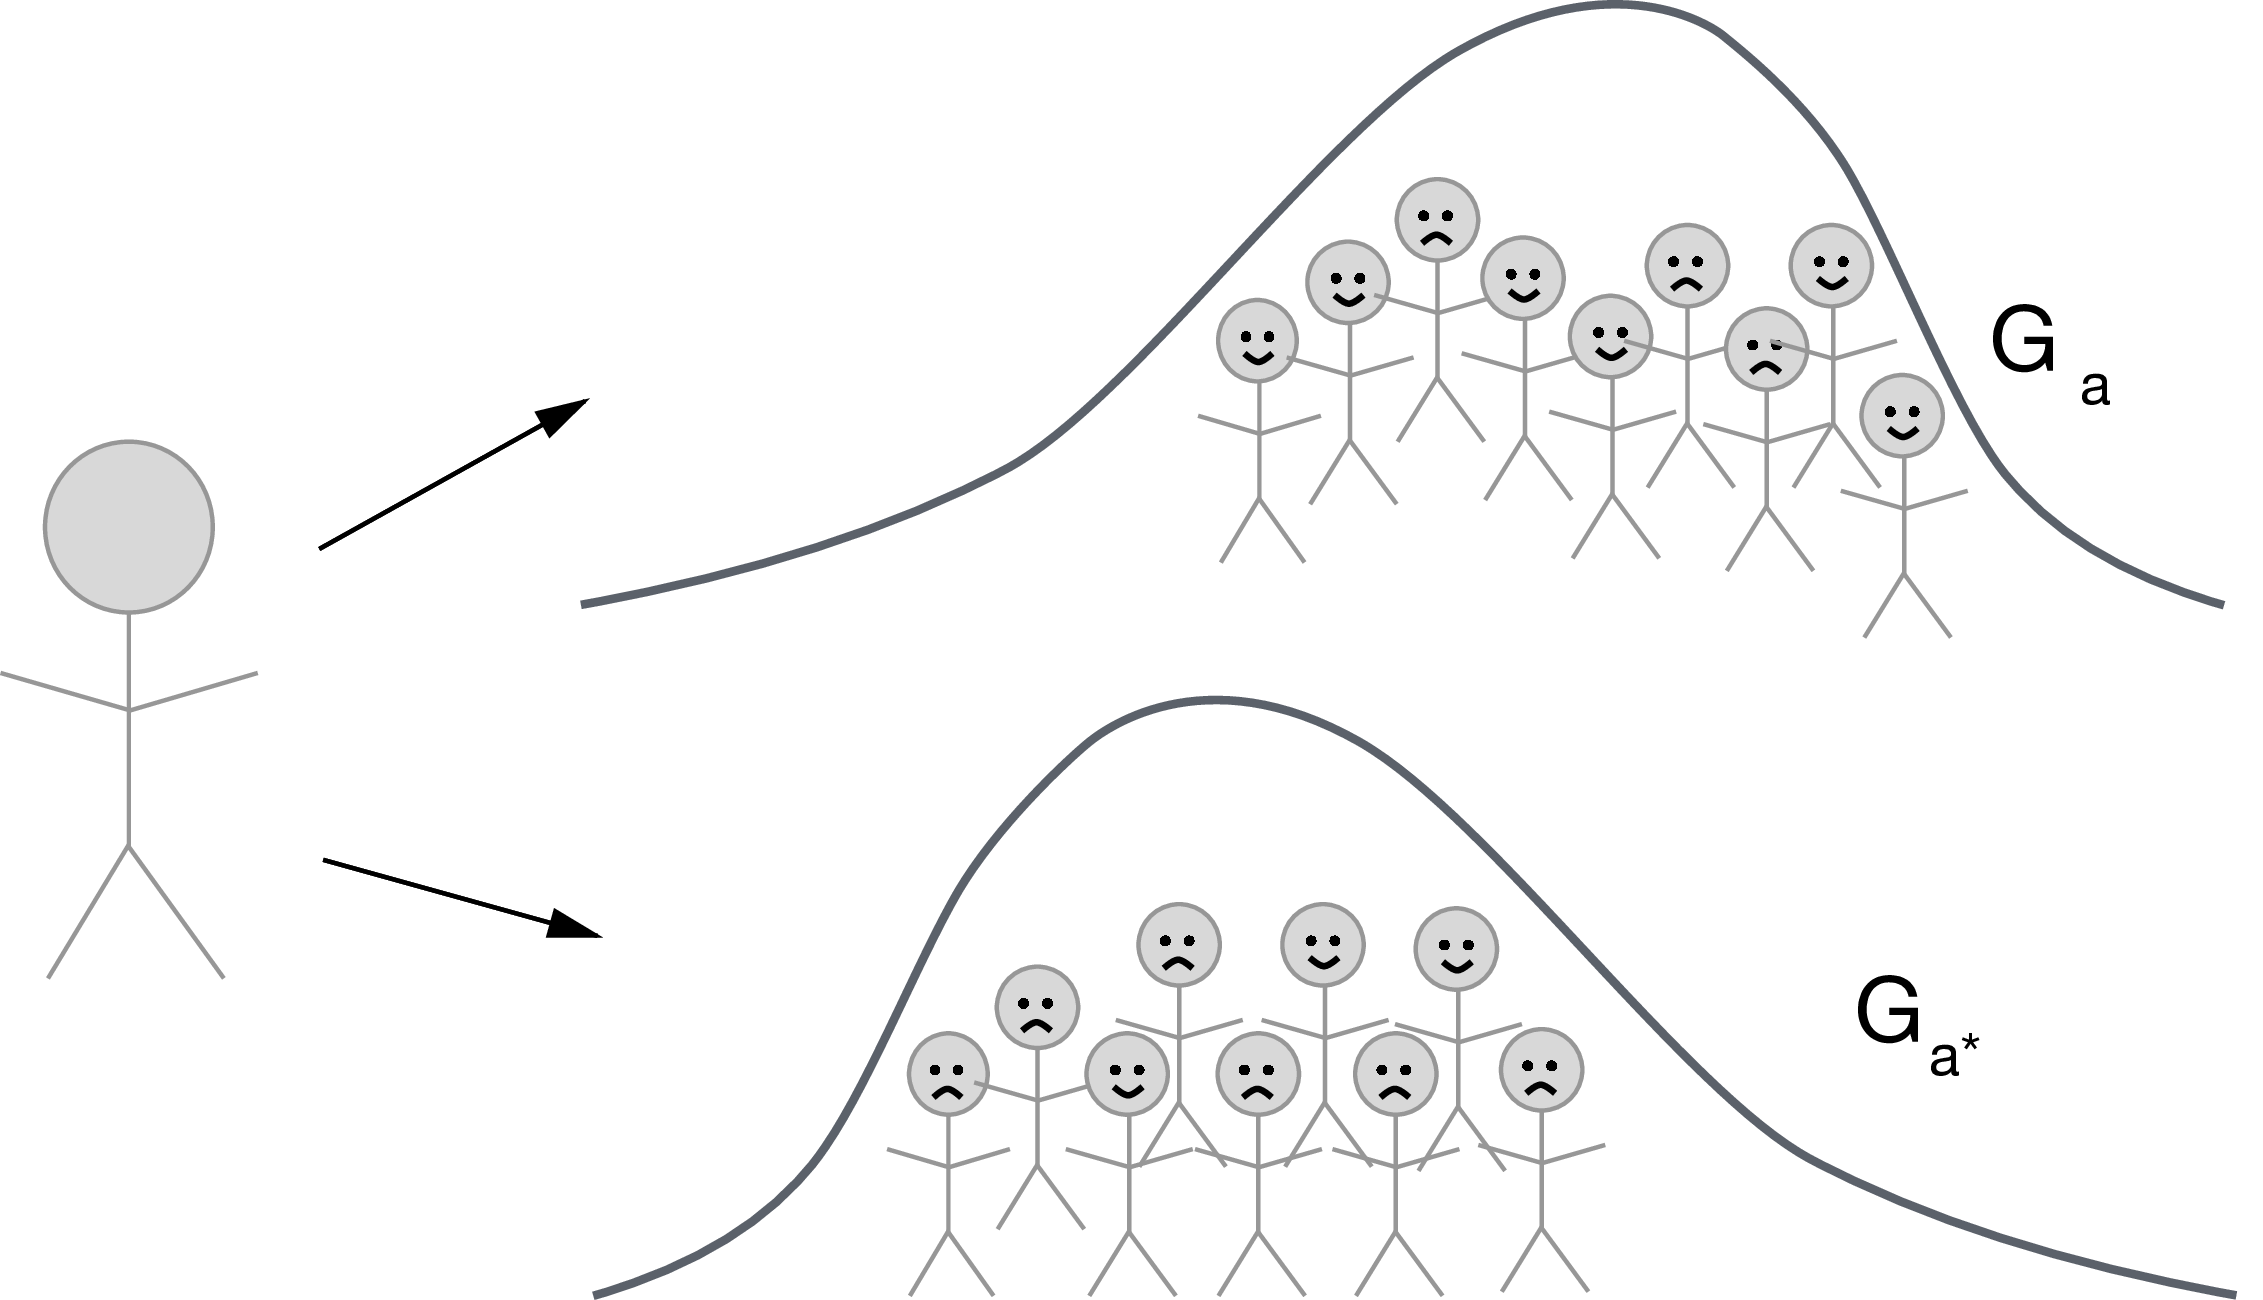
\includegraphics[width=0.5\linewidth]{/home/runner/work/ser2021_mediation_workshop/ser2021_mediation_workshop/img/graphic4b} 

}

\end{figure}

\hypertarget{an-alternative-definition-of-the-effects}{%
\subsection{An alternative definition of the effects:}\label{an-alternative-definition-of-the-effects}}

\begin{itemize}
\tightlist
\item
  Above we defined \(G_a\) as a random draw from the distribution of \(M_a \mid W\)
\item
  What if instead we define \(G_a\) as a random draw from the distribution of \(M_a \mid (Z_a,W)\)
\item
  It turns out the indirect effect defined in this way only measures the path
  \(A\rightarrow M \rightarrow Y\), and not the path \(A\rightarrow Z\rightarrow M \rightarrow Y\)
\item
  There may be important reasons to choose one over another (e.g., survival
  analyses where we want the distribution conditional on \(Z\), instrumental
  variable designs where it doesn't make sense to condition on \(Z\))
\end{itemize}

\hypertarget{identification-assumptions-2}{%
\subsection{Identification assumptions:}\label{identification-assumptions-2}}

\begin{itemize}
\tightlist
\item
  \(A \indep Y_{a,m} \mid W\)
\item
  \(M \indep Y_{a,m} \mid W, A, Z\)
\item
  \(A \indep M_a \mid W\)
\item
  and positivity assumptions.
\end{itemize}

Under these assumptions, the population interventional direct and indirect effect is identified:
\begin{align*}
  \E&(Y_{a, G_{a'}}) = \\
    &\E\left[\color{Purple}{\E\left\{\color{Goldenrod}{\sum_z}
    \color{ForestGreen}{\E(Y \mid A=a, Z=z, M, W)}
    \color{Goldenrod}{\P(Z=z \mid A=a, W)}\mid A=a', W\right\}}\right]
\end{align*}

\begin{itemize}
\tightlist
\item
  Let's dissect this formula in \passthrough{\lstinline!R!}:
\end{itemize}

\begin{lstlisting}[language=R]
n <- 1e6
w <- rnorm(n)
a <- rbinom(n, 1, 0.5)
z <- rbinom(n, 1, 0.5 + 0.2 * a)
m <- rnorm(n, w + a - z)
y <- rnorm(n, w + a + z + m)
\end{lstlisting}

\begin{itemize}
\tightlist
\item
  Let us compute \(\E(Y_{1, G_0})\) (so that \(a = 1\), and \(a'=0\)).
\item
  First, fit a regression model for the outcome, and compute
  \[\color{ForestGreen}{\E(Y \mid A=a, Z=z, M, W)}\] for all values of \(z\)
\end{itemize}

\begin{lstlisting}[language=R]
lm_y <- lm(y ~ m + a + z + w)
pred_a1z0 <- predict(lm_y, newdata = data.frame(m = m, a = 1, z = 0, w = w))
pred_a1z1 <- predict(lm_y, newdata = data.frame(m = m, a = 1, z = 1, w = w))
\end{lstlisting}

\begin{itemize}
\tightlist
\item
  Now we fit the true model for \(Z \mid A, W\) and get the conditional
  probability that \(Z=1\) fixing \(A=1\)
\end{itemize}

\begin{lstlisting}[language=R]
prob_z <- lm(z ~ a)
pred_z <- predict(prob_z, newdata = data.frame(a = 1))
\end{lstlisting}

\begin{itemize}
\tightlist
\item
  Now we compute the following pseudo-outcome:
  \[\color{Goldenrod}{\sum_z}\color{ForestGreen}{\E(Y \mid A=a, Z=z, M, W)}
  \color{Goldenrod}{\P(Z=z \mid A=a, w)}\]
\end{itemize}

\begin{lstlisting}[language=R]
pseudo_out <- pred_a1z0 * (1 - pred_z) + pred_a1z1 * pred_z
\end{lstlisting}

\begin{itemize}
\tightlist
\item
  Now we regress this pseudo-outcome on \(A,W\), and compute the predictions
  setting \(A=0\), that is, \[\color{Purple}{\E\left\{\color{Goldenrod}{\sum_z}
  \color{ForestGreen}{\E(Y \mid A=a, Z=z, M, W)}
  \color{Goldenrod}{\P(Z=z \mid A=a, w)}\mid A=a', W\right\}}\]
\end{itemize}

\begin{lstlisting}[language=R]
fit_pseudo <- lm(pseudo_out ~ a + w)
pred_pseudo <- predict(fit_pseudo, data.frame(a = 0, w = w))
\end{lstlisting}

\begin{itemize}
\tightlist
\item
  And finally, just average those predictions!
\end{itemize}

\begin{lstlisting}[language=R]
## Mean(Y(1, G(0)))
mean(pred_pseudo)
#> [1] 1.1979
\end{lstlisting}

\begin{itemize}
\tightlist
\item
  This was for \((a,a')=(1,0)\). Can do the same with \((a,a')=(1,1)\), and
  \((a,a')=(0,0)\) to obtain an effect decomposition
\end{itemize}

\begin{equation*}
  \E[Y_{1,G_1} - Y_{0,G_0}] = \underbrace{\E[Y_{\color{red}{1},
    \color{blue}{G_1}} -
    Y_{\color{red}{1},
    \color{blue}{G_0}}]}_{\text{interventional indirect effect}} +
    \underbrace{\E[Y_{\color{blue}{1},\color{red}{G_0}} -
    Y_{\color{blue}{0},
    \color{red}{G_0}}]}_{\text{interventional direct effect}}
\end{equation*}

\hypertarget{is-this-the-estimand-i-want-2}{%
\subsection{Is this the estimand I want?}\label{is-this-the-estimand-i-want-2}}

\begin{itemize}
\tightlist
\item
  Makes sense to intervene on \(A\) but not directly on \(M\).
\item
  Goal is to understand a natural mechanism underlying an association or total
  effect.
\item
  Okay with the assumptions!
\end{itemize}

\hypertarget{estimand-summary}{%
\section{Estimand Summary}\label{estimand-summary}}

\begin{figure}

{\centering 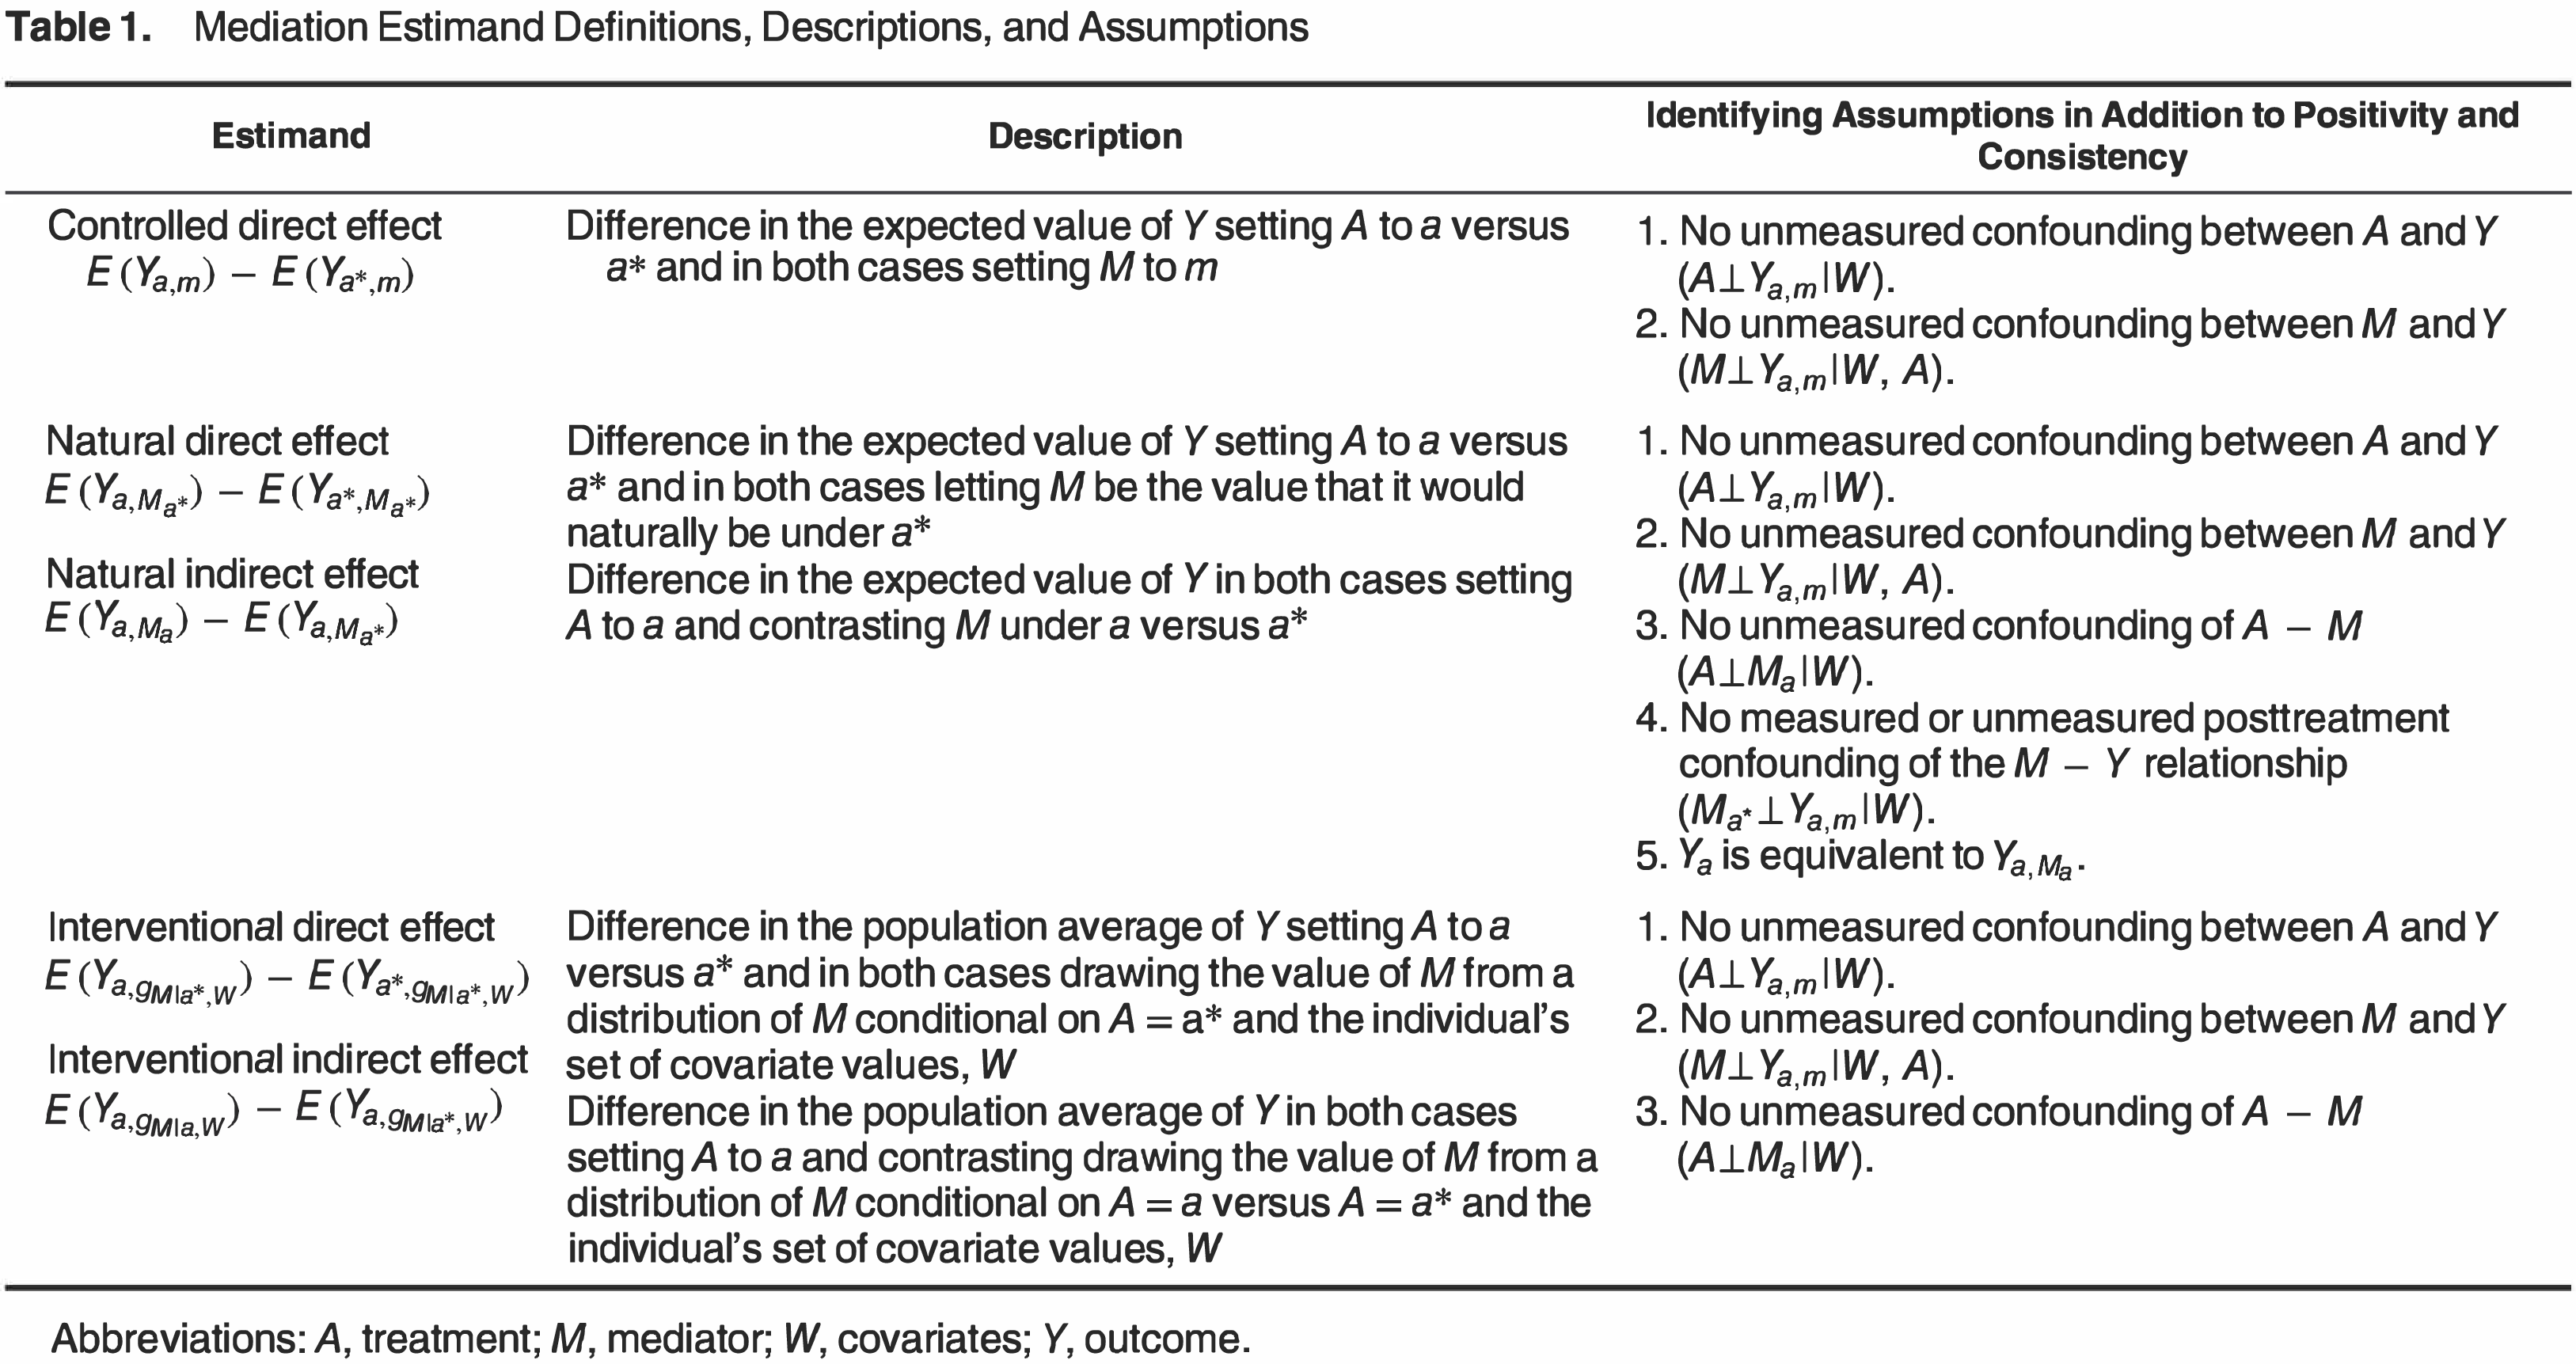
\includegraphics[width=1.25\linewidth]{/home/runner/work/ser2021_mediation_workshop/ser2021_mediation_workshop/img/table1} 

}

\end{figure}

\hypertarget{stochastic}{%
\chapter{Stochastic Direct and Indirect Effects}\label{stochastic}}

\hypertarget{definition-of-the-effects}{%
\section{Definition of the effects}\label{definition-of-the-effects}}

Consider the following directed acyclic graph.

\begin{figure}

{\centering \includegraphics[width=0.8\linewidth]{03-stochastic_files/figure-latex/unnamed-chunk-1-1} 

}

\caption{Directed acyclic graph under no intermediate confounders of the mediator-outcome relation affected by treatment}\label{fig:unnamed-chunk-1}
\end{figure}

\hypertarget{motivation-for-stochastic-interventions}{%
\section{Motivation for stochastic interventions}\label{motivation-for-stochastic-interventions}}

\begin{itemize}
\tightlist
\item
  So far we have discussed controlled, natural, and interventional (in)direct effects
\item
  These effects require that \(0 < \P(A=1\mid W) < 1\)
\item
  They are defined only for binary exposures
\item
  \emph{What can we do when the positivity assumption does not hold or the exposure
  is continuous?}
\item
  Solution: we can use stochastic effects
\end{itemize}

\hypertarget{definition-of-stochastic-effects}{%
\section{Definition of stochastic effects}\label{definition-of-stochastic-effects}}

There are two possible ways of defining stochastic effects:

\begin{itemize}
\tightlist
\item
  Consider the effect of an intervention where the exposure is drawn from a
  distribution

  \begin{itemize}
  \tightlist
  \item
    For example incremental propensity score interventions
  \end{itemize}
\end{itemize}

\begin{itemize}
\tightlist
\item
  Consider the effect of an intervention where the post-intervention exposure is
  a function of the actually received exposure

  \begin{itemize}
  \tightlist
  \item
    For example modified treatment policies
  \end{itemize}
\item
  In both cases \(A \mid W\) is a non-deterministic intervention, thus the name
  \emph{stochastic intervention}
\end{itemize}

\hypertarget{example-incremental-propensity-score-interventions-ipsi-kennedy2018nonparametric}{%
\subsection*{\texorpdfstring{Example: incremental propensity score interventions (IPSI) \citep{kennedy2018nonparametric}}{Example: incremental propensity score interventions (IPSI) {[}@kennedy2018nonparametric{]}}}\label{example-incremental-propensity-score-interventions-ipsi-kennedy2018nonparametric}}


\hypertarget{definition-of-the-intervention}{%
\subsubsection*{Definition of the intervention}\label{definition-of-the-intervention}}


\begin{itemize}
\tightlist
\item
  Assume \(A\) is binary, and \(\P(A=1\mid W=w) = g(1\mid w)\) is the propensity score
\item
  Consider an intervention in which each individual receives the intervention
  with probability \(g_\delta(1\mid w)\), equal to
  \begin{equation*}
    g_\delta(1\mid w)=\frac{\delta g(1\mid w)}{\delta g(1\mid w) +
    1 - g(1\mid w)}
  \end{equation*}
\item
  e.g., draw the post-intervention exposure from a Bernoulli variable with
  probability \(g_\delta(1\mid w)\)
\item
  The value \(\delta\) is user given
\item
  Let \(A_\delta\) denote the post-intervention exposure distribution
\item
  Some algebra shows that \(\delta\) is an odds ratio comparing the pre- and
  post-intervention exposure distributions
  \begin{equation*}
    \delta = \frac{\text{odds}(A_\delta = 1\mid W=w)}
    {\text{odds}(A = 1\mid W=w)}
  \end{equation*}
\item
  Interpretation: \emph{what would happen in a
  world where the odds of receiving treatment is increased by \(\delta\)}
\item
  Let \(Y_{A_\delta}\) denote the outcome in this hypothetical world
\end{itemize}

\hypertarget{illustrative-application-for-ipsis}{%
\subsubsection{Illustrative application for IPSIs}\label{illustrative-application-for-ipsis}}

\begin{itemize}
\tightlist
\item
  Consider the effect of participation in sports on children's BMI
\item
  Mediation through snacking, exercising, etc.
\item
  Intervention: for each individual, increase the odds of participating in
  sports by \(\delta=2\)
\item
  The post-intervention exposure is a draw \(A_\delta\) from a Bernoulli
  distribution with probability \(g_\delta(1\mid w)\)
\end{itemize}

\hypertarget{example-modified-treatment-policies-mtp-diaz2020causal}{%
\subsection*{\texorpdfstring{Example: modified treatment policies (MTP) \citep{diaz2020causal}}{Example: modified treatment policies (MTP) {[}@diaz2020causal{]}}}\label{example-modified-treatment-policies-mtp-diaz2020causal}}


\hypertarget{definition-of-the-intervention-1}{%
\subsubsection*{Definition of the intervention}\label{definition-of-the-intervention-1}}


\begin{itemize}
\tightlist
\item
  Consider a continuous exposure \(A\) taking values in the real numbers
\item
  Consider an intervention that assigns exposure as \(A_\delta = A - \delta\)
\item
  Example: \(A\) is pollution measured as \(PM_{2.5}\) and you are interested in an
  intervention that reduces \(PM_{2.5}\) concentration by some amount \(\delta\)
\end{itemize}

\hypertarget{mediation-analysis-for-stochastic-interventions}{%
\subsection{Mediation analysis for stochastic interventions}\label{mediation-analysis-for-stochastic-interventions}}

\begin{itemize}
\item
  The total effect of an IPSI can be computed as a contrast of the outcome under
  intervention vs no intervention:
  \begin{equation*}
    \psi = \E[Y_{A_\delta} - Y]
  \end{equation*}
\item
  Recall the NPSEM
  \begin{align}
    W & = f_W(U_W)\\
    A & = f_A(W, U_A)\\
    M & = f_M(W, A, U_M)\\
    Y & = f_Y(W, A, M, U_Y)
  \end{align}
\item
  From this we have
  \begin{align*}
  M_{A_\delta} & = f_M(W, A_\delta, U_M)\\
  Y_{A_\delta} & = f_Y(W, A_\delta, M_{A_\delta}, U_Y)
  \end{align*}
\item
  Thus, we have \(Y_{A_\delta} = Y_{A_\delta, M_{A_\delta}}\) and \(Y = Y_{A,M_{A}}\)
\item
  Let us introduce the counterfactual \(Y_{A_\delta, M}\), interpreted as the
  outcome observed in a world where the intervention on \(A\) is performed but the
  mediator is fixed at the value it would have taken under no intervention:
  \[Y_{A_\delta, M}  = f_Y(W, A_\delta, M_{A_\delta}, U_Y)\]
\item
  Then we can decompose the total effect into:
  \begin{align*}
    \E[Y&_{A_\delta,M_{A_\delta}} - Y_{A,M_A}] = \\
    &\underbrace{\E[Y_{\color{red}{A_\delta},\color{blue}{M_{A_\delta}}} -
      Y_{\color{red}{A_\delta},\color{blue}{M}}]}_{\text{stochastic natural indirect effect}} +
      \underbrace{\E[Y_{\color{blue}{A_\delta},\color{red}{M}} -
      Y_{\color{blue}{A},\color{red}{M}}]}_{\text{stochastic natural direct effect}}
  \end{align*}
\end{itemize}

\hypertarget{identification-assumptions-3}{%
\section{Identification assumptions}\label{identification-assumptions-3}}

\begin{itemize}
\tightlist
\item
  Confounder assumptions:

  \begin{itemize}
  \tightlist
  \item
    \(A \indep Y_{a,m} \mid W\)
  \item
    \(M \indep Y_{a,m} \mid W, A\)
  \end{itemize}
\item
  No confounder of \(M\rightarrow Y\) affected by \(A\)
\item
  Positivity assumptions:

  \begin{itemize}
  \tightlist
  \item
    If \(g_\delta(a \mid w)>0\) then \(g(a \mid w)>0\)
  \item
    If \(\P(Z=z\mid W=w)>0\) then \(\P(Z=z\mid A=a,W=w)>0\)
  \end{itemize}
\end{itemize}

Under these assumptions, stochastic effects are identified as follows

\begin{itemize}
\item
  The indirect effect can be identified as follows
  \begin{align*}
  \E&(Y_{A_\delta} - Y_{A_\delta, M}) =\\
  &\E\left[\color{Goldenrod}{\sum_{a}\color{ForestGreen}{\{\E(Y\mid A=a, W)-\E(Y\mid A=a, M, W)\}}g_\delta(a\mid W)}\right]
  \end{align*}
\item
  The direct effect can be identified as follows
  \begin{align*}
  \E&(Y_{A_\delta} - Y_{A_\delta, M}) =\\
  &\E\left[\color{Goldenrod}{\sum_{a}\color{ForestGreen}{\{\E(Y\mid A=a, M, W) - Y\}}g_\delta(a\mid W)}\right]
  \end{align*}
\item
  Let's dissect the formula for the indirect effect in R:
\end{itemize}

\begin{lstlisting}[language=R]
n <- 1e6
w <- rnorm(n)
a <- rbinom(n, 1, plogis(1 + w))
m <- rnorm(n, w + a)
y <- rnorm(n, w + a + m)
\end{lstlisting}

\begin{itemize}
\tightlist
\item
  First, fit regressions of the outcome on \((A,W)\) and \((M,A,W)\):
\end{itemize}

\begin{lstlisting}[language=R]
fit_y1 <- lm(y ~ m + a + w)
fit_y2 <- lm(y ~ a + w)
\end{lstlisting}

\begin{itemize}
\tightlist
\item
  Get predictions fixing \(A=a\) for all possible values \(a\)
\end{itemize}

\begin{lstlisting}[language=R]
pred_y1_a1 <- predict(fit_y1, newdata = data.frame(a = 1, m, w))
pred_y1_a0 <- predict(fit_y1, newdata = data.frame(a = 0, m, w))
pred_y2_a1 <- predict(fit_y2, newdata = data.frame(a = 1, w))
pred_y2_a0 <- predict(fit_y2, newdata = data.frame(a = 0, w))
\end{lstlisting}

\begin{itemize}
\tightlist
\item
  Compute
  \[\color{ForestGreen}{\{\E(Y\mid A=a, W)-\E(Y\mid A=a, M, W)\}}\]
  for each value \(a\)
\end{itemize}

\begin{lstlisting}[language=R]
pseudo_a1 <- pred_y2_a1 - pred_y1_a1
pseudo_a0 <- pred_y2_a0 - pred_y1_a0
\end{lstlisting}

\begin{itemize}
\tightlist
\item
  Estimate the propensity score \(g(1\mid w)\) and evaluate the post-intervention
  propensity score \(g_\delta(1\mid w)\)
\end{itemize}

\begin{lstlisting}[language=R]
pscore_fit <- glm(a ~ w, family = binomial())
pscore <- predict(pscore_fit, type = 'response')
## How do the intervention vs observed propensity score compare
pscore_delta <- 2 * pscore / (2 * pscore + 1 - pscore)
\end{lstlisting}

\begin{itemize}
\tightlist
\item
  What do the post-intervention propensity scores look like?
\end{itemize}

\begin{lstlisting}[language=R]
plot(pscore, pscore_delta, xlab = 'Observed prop. score',
     ylab = 'Prop. score under intervention')
abline(0, 1)
\end{lstlisting}

\begin{center}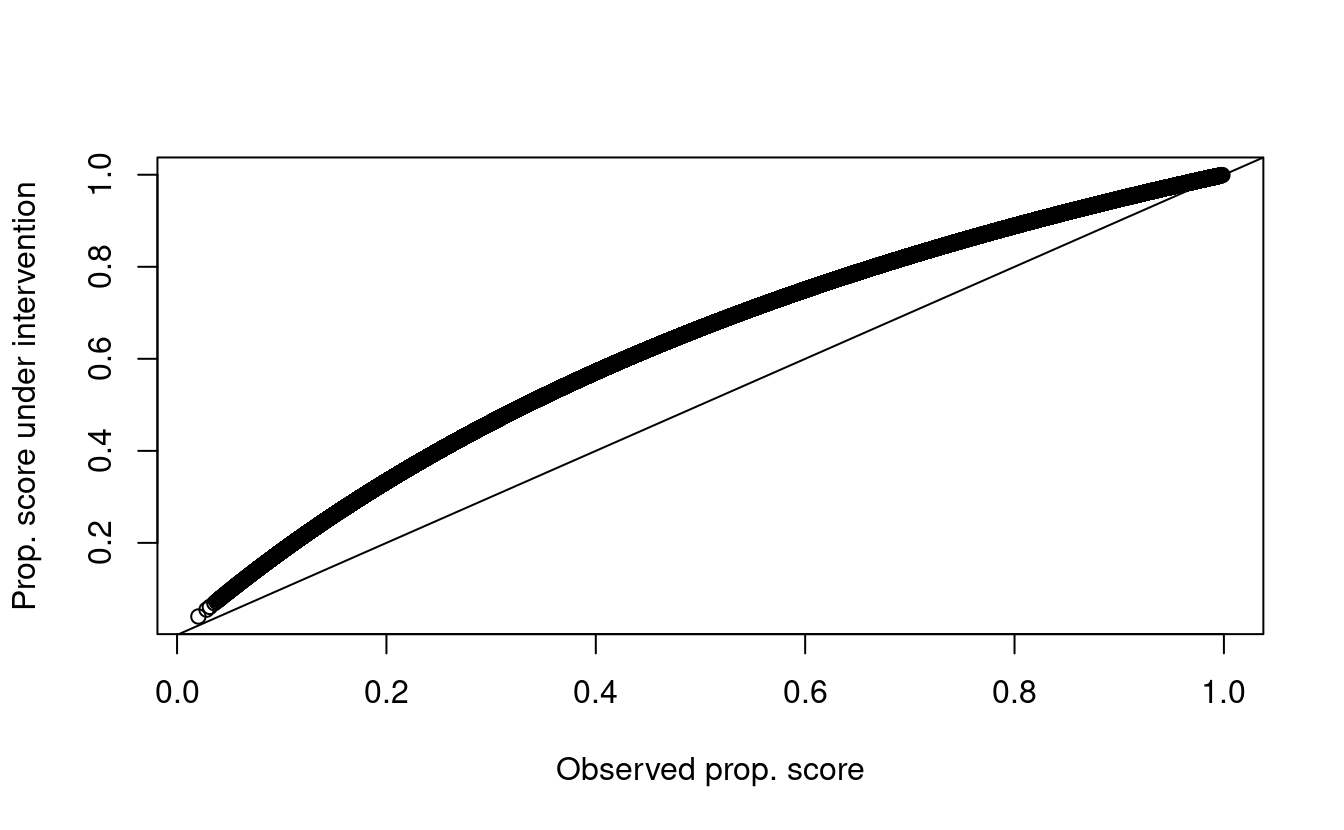
\includegraphics[width=0.8\linewidth]{03-stochastic_files/figure-latex/unnamed-chunk-7-1} \end{center}

\hypertarget{what-are-the-odds-of-exposure-under-intervention-vs-real-world}{%
\section{What are the odds of exposure under intervention vs real world?}\label{what-are-the-odds-of-exposure-under-intervention-vs-real-world}}

\begin{lstlisting}[language=R]
odds <- (pscore_delta / (1 - pscore_delta)) / (pscore / (1 - pscore))
summary(odds)
#>    Min. 1st Qu.  Median    Mean 3rd Qu.    Max. 
#>       2       2       2       2       2       2
\end{lstlisting}

\begin{itemize}
\tightlist
\item
  Compute the sum
  \[\color{Goldenrod}{\sum_{a}\color{ForestGreen}{\{\E(Y\mid A=a, W)-\E(Y\mid A=a, M, W)\}}g_\delta(a\mid W)}\]
\end{itemize}

\begin{lstlisting}[language=R]
indirect <- pseudo_a1 * pscore_delta + pseudo_a0 * (1 - pscore_delta)
\end{lstlisting}

\begin{itemize}
\tightlist
\item
  The average of this value is the indirect effect
\end{itemize}

\begin{lstlisting}[language=R]
## E[Y(Adelta) - Y(Adelta, M)]
mean(indirect)
#> [1] 0.1091
\end{lstlisting}

\begin{itemize}
\item
  The direct effect is
  \begin{align*}
  \E&(Y_{A_\delta} - Y_{A_\delta, M}) =\\
  &\E\left[\color{Goldenrod}{\sum_{a}\color{ForestGreen}{\{\E(Y\mid A=a, M, W) - Y\}}g_\delta(a\mid W)}\right]
  \end{align*}
\item
  Which can be computed as
\end{itemize}

\begin{lstlisting}[language=R]
direct <- (pred_y1_a1 - y) * pscore_delta +
       (pred_y1_a0 - y) * (1 - pscore_delta)
mean(direct)
#> [1] 0.10934
\end{lstlisting}

\hypertarget{summary}{%
\section{Summary}\label{summary}}

\begin{itemize}
\tightlist
\item
  Stochastic (in)direct effects

  \begin{itemize}
  \tightlist
  \item
    Relax the positivity assumption
  \item
    Can be defined for non-binary exposures
  \item
    Do not require a cross-world assumption
  \end{itemize}
\item
  Still require the absence of intermediate confounders

  \begin{itemize}
  \tightlist
  \item
    But, compared to the NDE and NIE, we can design a randomized study where
    identifiability assumptions hold, at least in principle
  \item
    There is a version of these effects that can accomodate intermediate
    confounders \citep{hejazi2020nonparametric}
  \item
    \passthrough{\lstinline!R!} implementation to be released soon\ldots stay tuned!
  \end{itemize}
\end{itemize}

\hypertarget{estimandirl}{%
\chapter{How to choose an estimand: Real world example}\label{estimandirl}}

\hypertarget{comparative-effectivness-of-two-medications-for-opioid-use-disorder-oud}{%
\section{Comparative effectivness of two medications for opioid use disorder (OUD)}\label{comparative-effectivness-of-two-medications-for-opioid-use-disorder-oud}}

\begin{figure}

{\centering 
\includegraphics[width=1\linewidth]{/home/runner/work/ser2021_mediation_workshop/ser2021_mediation_workshop/img/ctndag} 

}

\end{figure}

\emph{Motivation}: Opposite overall treatment effects for homeless versus
nonhomeless participants.

\begin{figure}

{\centering 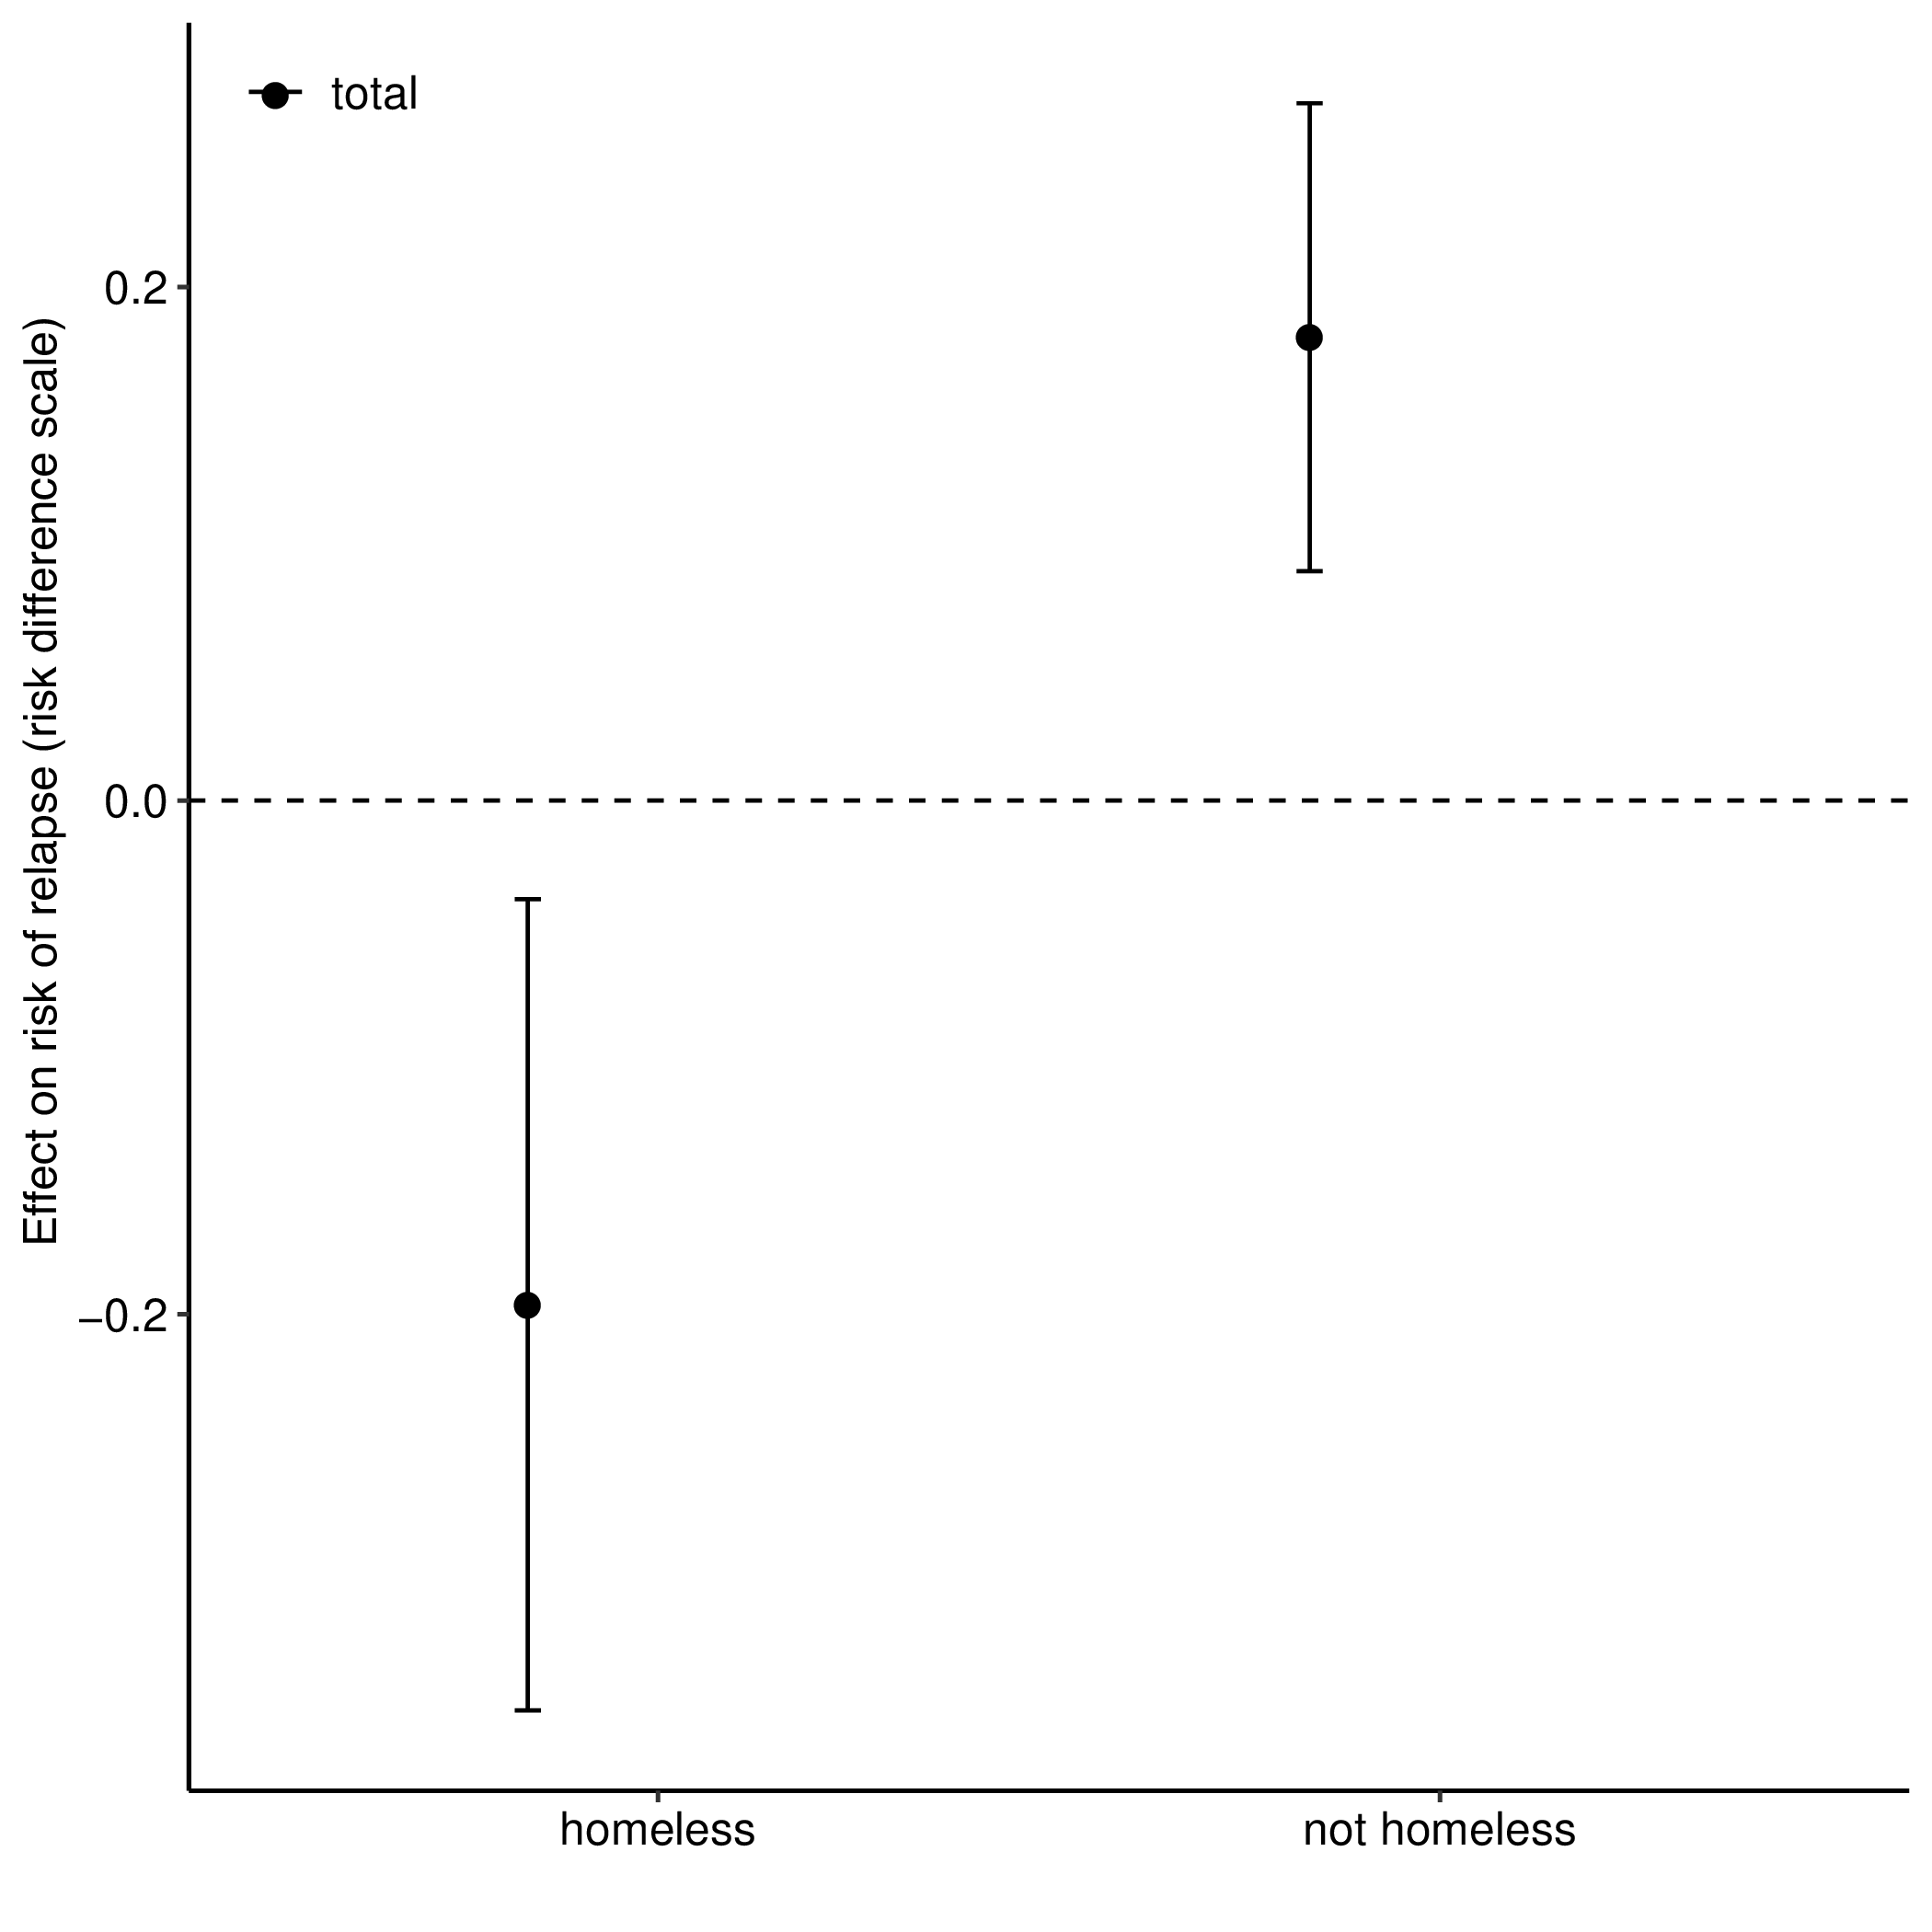
\includegraphics[width=0.5\linewidth]{/home/runner/work/ser2021_mediation_workshop/ser2021_mediation_workshop/img/tmleesttotal} 

}

\end{figure}

\hypertarget{getting-specific-about-the-question}{%
\subsection{Getting specific about the question}\label{getting-specific-about-the-question}}

To what extent does the indirect effect through mediators of adherence, pain, and
depressive symptoms explain the differences in treatment effects on OUD relapse
for homeless and nonhomeless individuals?

\hypertarget{what-estimand-do-we-want}{%
\subsubsection*{What estimand do we want?}\label{what-estimand-do-we-want}}


\begin{itemize}
\tightlist
\item
  Can we set \(M=m\) (i.e., same value) for everyone?
\item
  Are we interested in estimating indirect effects?
\end{itemize}

\(\rightarrow\) So, \emph{not} controlled direct effect.

\begin{itemize}
\tightlist
\item
  Do we have an intermediate confounder?
\item
  Yes, and it's important.
\end{itemize}

\(\rightarrow\) So, \emph{not} natural (in)direct effects.

\begin{itemize}
\tightlist
\item
  So, we're left with the interventional direct and indirect effects.
\item
  Do we want to estimate the path through treatment initiation (\(Z\))?
\item
  Yes, so, \emph{not} the conditional versions of these effects.
\item
  Estimands:

  \begin{itemize}
  \tightlist
  \item
    Direct effect: \(\E(Y_{1,G_0} - Y_{0,G_0})\)
  \item
    Indirect effect: \(\E(Y_{1,G_1} - Y_{1,G_0})\)
  \end{itemize}
\item
  Here \(G_a\) is a draw from the distribution of \(M_a\mid W\).
\item
  Need to incorporate multiple and continuous mediators
\end{itemize}

\hypertarget{what-if-the-positivity-assumption-paamid-w0-violated}{%
\subsubsection*{\texorpdfstring{What if the positivity assumption \(\P(A=a\mid W)>0\) violated?}{What if the positivity assumption \textbackslash P(A=a\textbackslash mid W)\textgreater0 violated?}}\label{what-if-the-positivity-assumption-paamid-w0-violated}}


\(\rightarrow\) Can't identify or estimate any of the above effects

\begin{itemize}
\tightlist
\item
  But we can estimate the effect of some stochastic interventions, e.g., IPSIs
\item
  Tradeoff between feasibility and interpretation
\end{itemize}

\hypertarget{what-if-the-exposure-variable-is-continuous}{%
\subsubsection*{What if the exposure variable is continuous?}\label{what-if-the-exposure-variable-is-continuous}}


\(\rightarrow\) All the above effects are defined for binary exposures

\begin{itemize}
\tightlist
\item
  But we can estimate the effect of some stochastic interventions
\item
  Work in progress (including upcoming R software)
\end{itemize}

\hypertarget{preliminaries-on-semiparametric-estimation}{%
\chapter{Preliminaries on semiparametric estimation}\label{preliminaries-on-semiparametric-estimation}}

\hypertarget{from-causal-to-statistical-quantities}{%
\section{From causal to statistical quantities}\label{from-causal-to-statistical-quantities}}

\begin{itemize}
\tightlist
\item
  We have arrived at identification formulas that express quantities that we
  care about in terms of observable quantities
\item
  This required \textbf{causal assumptions}

  \begin{itemize}
  \tightlist
  \item
    Many of these assumptions are empirically unverifiable
  \item
    We saw an example where we could relax the cross-world assumption, at the
    cost of changing the parameter interpretation
  \item
    and where we could relax the positivity assumption, also at the cost of
    changing the parameter interpretation
  \end{itemize}
\item
  The resulting estimation problem can be tackled using \textbf{statistical
  assumptions} of various degrees of strength

  \begin{itemize}
  \tightlist
  \item
    Most of these assumptions are verifiable (e.g., a linear model)
  \item
    Thus, most are unnecessary (except for convenience)
  \item
    The estimation approach we use reduces reliance on these statistical
    assumptions
  \end{itemize}
\end{itemize}

\hypertarget{computing-identification-formulas-if-you-know-the-true-distribution}{%
\subsection{Computing identification formulas if you know the true distribution}\label{computing-identification-formulas-if-you-know-the-true-distribution}}

\begin{itemize}
\tightlist
\item
  The mediation parameters that we consider can be
  seen as a function of the joint probability distribution of \(O=(W,A,Z,M,Y)\)
\item
  For example, under identifiability assumptions the natural direct effect is
  equal to
  \begin{equation*}
    \psi(\P) =  \E[\E\{\E(Y \mid A=1, M, W) - \E(Y \mid A=0, M, W)\mid A=0,W\}]
  \end{equation*}
\item
  The notation \(\psi(\P)\) implies that the parameter is a function of \(\P\)
\item
  This means that we can compute it for any distribution \(\P\)
\item
  For example, if we know the true \(\P(W,A,M,Y)\), we can comnpute the true value
  of the parameter by:

  \begin{itemize}
  \tightlist
  \item
    Computing the conditional expectation \(\E(Y\mid A=1,M=m,W=w)\) for all
    values \((m,w)\)
  \item
    Computing the probability \(\P(M=m\mid A=0,W=w)\) for all values \((m,w)\)
  \item
    Computing the probability \(\P(W=w)\) for all values \(w\)
  \item
    Computing the mean over all values \((m,w)\)
  \end{itemize}
\end{itemize}

\hypertarget{estimating-identification-formulas}{%
\subsection{Estimating identification formulas}\label{estimating-identification-formulas}}

The above is how you would compute the \emph{true value} \textbf{if you know} the true
distribution \(\P\)

\begin{itemize}
\tightlist
\item
  This is exactly what we did in our R examples before
\item
  But we can use the same logic for estimation:

  \begin{itemize}
  \tightlist
  \item
    Fit a regression to estimate, say \(\hat\E(Y\mid A=1,M=m,W=w)\)
  \item
    Fit a regression to estimate, say \(\hat\P(M=m\mid A=0,W=w)\)
  \item
    Estimate \(\P(W=w)\) with the empirical distribution
  \item
    Evaluate
    \begin{equation*}
      \psi(\hat\P) =  \hat\E[\hat\E\{\hat\E(Y \mid A=1, M, W) -
      \hat\E(Y \mid A=0, M, W)\mid A=0,W\}]
    \end{equation*}
  \end{itemize}
\item
  This is known as the g-computation estimator
\end{itemize}

\hypertarget{how-can-g-estimation-be-implemented-in-practice}{%
\subsection{How can g-estimation be implemented in practice?}\label{how-can-g-estimation-be-implemented-in-practice}}

\begin{itemize}
\tightlist
\item
  There are two possible ways to do g-computation estimation:

  \begin{itemize}
  \tightlist
  \item
    Using parametric models for the above regressions
  \item
    Using flexible data-adaptive regression (aka machine learning)
  \end{itemize}
\end{itemize}

\hypertarget{pros-and-cons-of-parametric-models}{%
\subsection{Pros and cons of parametric models}\label{pros-and-cons-of-parametric-models}}

\begin{itemize}
\tightlist
\item
  Pros:

  \begin{itemize}
  \tightlist
  \item
    Easy to understand
  \item
    Ease of implementation (standard regression software)
  \item
    Can use the Delta method or the bootstrap for computation of standard errors
  \end{itemize}
\item
  Cons:

  \begin{itemize}
  \tightlist
  \item
    Unless \(W\) and \(M\) contain very few categorical variables, it is very easy
    to misspecify the models
  \item
    This can introduce sizable bias in the estimators
  \end{itemize}
\end{itemize}

\hypertarget{an-example-of-the-bias-of-a-g-computation-estimator-of-the-natural-direct-effect}{%
\subsection{An example of the bias of a g-computation estimator of the natural direct effect}\label{an-example-of-the-bias-of-a-g-computation-estimator-of-the-natural-direct-effect}}

\begin{itemize}
\tightlist
\item
  The following \passthrough{\lstinline!R!} chunk provides simulation code to exemplify the bias of a
  g-computation estimator in a simple situation
\end{itemize}

\begin{lstlisting}[language=R]
mean_y <- function(m, a, w) abs(w) + a * m
mean_m <- function(a, w) plogis(w^2 - a)
pscore <- function(w) plogis(1 - abs(w))
\end{lstlisting}

\begin{itemize}
\tightlist
\item
  This yields a true NDE value of
\end{itemize}

\begin{lstlisting}[language=R]
w_big <- runif(1e6, -1, 1)
trueval <- mean((mean_y(1, 1, w_big) - mean_y(1, 0, w_big)) *
  mean_m(0, w_big) + (mean_y(0, 1, w_big) - mean_y(0, 0, w_big)) *
    (1 - mean_m(0, w_big)))
print(trueval)
#> [1] 0.58048
\end{lstlisting}

\begin{itemize}
\tightlist
\item
  Let's perform a simulation where we draw 1000 datasets from the above
  distribution, and compute a g-computation estimator based on
\end{itemize}

\begin{lstlisting}[language=R]
gcomp <- function(y, m, a, w) {
  lm_y <- lm(y ~ m + a + w)
  pred_y1 <- predict(lm_y, newdata = data.frame(a = 1, m = m, w = w))
  pred_y0 <- predict(lm_y, newdata = data.frame(a = 0, m = m, w = w))
  pseudo <- pred_y1 - pred_y0
  lm_pseudo <- lm(pseudo ~ a + w)
  pred_pseudo <- predict(lm_pseudo, newdata = data.frame(a = 0, w = w))
  estimate <- mean(pred_pseudo)
  return(estimate)
}
\end{lstlisting}

\begin{lstlisting}[language=R]
estimate <- lapply(seq_len(1000), function(iter) {
  n <- 1000
  w <- runif(n, -1, 1)
  a <- rbinom(n, 1, pscore(w))
  m <- rbinom(n, 1, mean_m(a, w))
  y <- rnorm(n, mean_y(m, a, w))
  est <- gcomp(y, m, a, w)
  return(est)
})
estimate <- do.call(c, estimate)

hist(estimate)
abline(v = trueval, col = "red", lwd = 4)
\end{lstlisting}

\begin{center}\includegraphics[width=0.8\linewidth]{05-preliminaries-estimation_files/figure-latex/unnamed-chunk-4-1} \end{center}

\begin{itemize}
\tightlist
\item
  The bias also affects the confidence intervals:
\end{itemize}

\begin{lstlisting}[language=R]
cis <- cbind(
  estimate - qnorm(0.975) * sd(estimate),
  estimate + qnorm(0.975) * sd(estimate)
)

ord <- order(rowSums(cis))
lower <- cis[ord, 1]
upper <- cis[ord, 2]
curve(trueval + 0 * x,
  ylim = c(0, 1), xlim = c(0, 1001), lwd = 2, lty = 3, xaxt = "n",
  xlab = "", ylab = "Confidence interval", cex.axis = 1.2, cex.lab = 1.2
)
for (i in 1:1000) {
  clr <- rgb(0.5, 0, 0.75, 0.5)
  if (upper[i] < trueval || lower[i] > trueval) clr <- rgb(1, 0, 0, 1)
  points(rep(i, 2), c(lower[i], upper[i]), type = "l", lty = 1, col = clr)
}
text(450, 0.10, "n=1000 repetitions = 1000 ", cex = 1.2)
text(450, 0.01, paste0(
  "Coverage probability = ",
  mean(lower < trueval & trueval < upper), "%"
), cex = 1.2)
\end{lstlisting}

\begin{center}\includegraphics[width=0.8\linewidth]{05-preliminaries-estimation_files/figure-latex/unnamed-chunk-5-1} \end{center}

\hypertarget{pros-and-cons-of-g-computation-with-data-adaptive-regression}{%
\subsection{Pros and cons of g-computation with data-adaptive regression}\label{pros-and-cons-of-g-computation-with-data-adaptive-regression}}

\begin{itemize}
\tightlist
\item
  Pros:

  \begin{itemize}
  \tightlist
  \item
    Easy to understand
  \item
    Alleviate model-misspecification bias
  \end{itemize}
\item
  Cons:

  \begin{itemize}
  \tightlist
  \item
    Might be harder to implement depending on the regression procedures used
  \item
    No general approaches for computation of standard errors and confidence
    intervals
  \item
    For example, the bootstrap is not guaranteed to work, and it is known to
    fail in some cases
  \end{itemize}
\end{itemize}

\hypertarget{semiparametric-estimation-or-correcting-the-bias-of-g-computation-estimators}{%
\section{Semiparametric estimation (or correcting the bias of g-computation estimators)}\label{semiparametric-estimation-or-correcting-the-bias-of-g-computation-estimators}}

\begin{itemize}
\tightlist
\item
  G-computation estimation with data-adaptive regression offers an incorrect
  bias/variance trade-off
\item
  It accepts more bias than necessary
\item
  The bias of a g-computation estimator may be corrected as follows:
  \begin{equation*}
    \psi(\hat \P) + \frac{1}{n}\sum_{i=1}^n D(O_i)
  \end{equation*}
  for some function \(D(O_i)\) of the data
\item
  The function \(D(O)\) is called \emph{the efficient influence function} (EIF)
\item
  The EIF must be found on a case-by-case basis for each parameter \(\psi(\P)\)
\item
  For example, for estimating the standardized mean \(\psi(\P)=\E[\E(Y\mid A=1, W)]\), we have
  \begin{equation*}
    D(O) = \frac{A}{\hat \P(A=1\mid W)}[Y - \hat\E(Y\mid A=1, W)] +
    \hat\E(Y\mid A=1, W) - \psi(\hat\P)
  \end{equation*}
\item
  The EIF is found by using a distributional analogue of a Taylor expansion
\item
  In this workshop we will omit the specific form of \(D(O)\) for
  some of the parameters that we use
\item
  But the estimators we discuss and implement in the R packages will be based on
  these EIFs
\item
  And the specific form of the EIF may be found in papers in the references
\end{itemize}

Note: the bias correction above may have an additional problem of returning
parameter estimates outside of natural bounds. E.g., probabilities greater than
one. A solution to this (not discussed in this workshop) is targeted minimum
loss based estimation.

\hypertarget{using-the-eif-to-construct-an-estimator-the-case-of-the-natural-direct-effect}{%
\chapter{Using the EIF to construct an estimator: the case of the natural direct effect}\label{using-the-eif-to-construct-an-estimator-the-case-of-the-natural-direct-effect}}

\hypertarget{natural-direct-effect}{%
\section{Natural direct effect}\label{natural-direct-effect}}

Recall:

\begin{figure}

{\centering \includegraphics[width=0.8\linewidth]{06-estimation-natural-interventional_files/figure-latex/unnamed-chunk-1-1} 

}

\caption{Directed acyclic graph under *no intermediate confounders* of the mediator-outcome relation affected by treatment}\label{fig:unnamed-chunk-1}
\end{figure}

\begin{itemize}
\item
  Assuming a binary \(A\), we define the natural direct effect as: \[NDE = E(Y_{1,M_{0}} - Y_{0,M_{0}}),\]
\item
  and the natural indirect effect as: \[NIE = E(Y_{1,M_{1}} - Y_{1,M_{0}}).\]
\item
  The observed data is \(O=(W, A, M, Y)\)
\end{itemize}

This SCM is represented in the above DAG and the following causal models:
\begin{align*}
  W & = f_W(U_W)\\
  A & = f_A(W, U_A)\\
  M & = f_M(W, A, U_M)\\
  Y & = f_Y(W, A, M, U_Y),
\end{align*}
where \((U_W, U_A,U_M, U_Y)\) are exogenous random errors.

We assume
- \(A\) is a single binary randomized treatment (and thus \(A = f_A(U_A)\))
- \(M\) is a single binary mediator
- There are no restrictions on the distribution of \(W\) or \(Y\)

Recall that we need to assume the following to identify the above caual effects
from our observed data:

\begin{itemize}
\tightlist
\item
  \(A \indep Y_{a,m} \mid W\)
\item
  \(M \indep Y_{a,m} \mid W, A\)
\item
  \(A \indep M_a \mid W\)
\item
  \(M_0 \indep Y_{1,m} \mid W\)
\item
  and positivity assumptions
\end{itemize}

Then, the NDE is identified as
\begin{equation*}
    \psi(\P) =  \E[\E\{\E(Y \mid A=1, M, W) - \E(Y \mid A=0, M, W)\mid A=0,W\}]
  \end{equation*}

\hypertarget{the-efficient-influence-function-for-the-nde}{%
\subsection{The efficient influence function for the NDE}\label{the-efficient-influence-function-for-the-nde}}

\begin{itemize}
\tightlist
\item
  For illustration, we will first present how to construct an estimator of the
  NDE that uses the EIF ``by hand''
\item
  For other parameters, we will teach you how to use our packages \emph{medoutcon}
  and \emph{medshift}
\end{itemize}

First, we need to introduce some notation to describe the EIF for the NDE

\begin{itemize}
\item
  Let \(Q(M, W)\) denote \(\E(Y\mid A=1, M, W) - \E(Y\mid A=0, M, W)\)
\item
  We can now introduce the EIF:
  \begin{align*}
    D(O) &= \color{ForestGreen}{\bigg\{ \frac{I(A=1)}{\P(A=1\mid W)}\frac{\P(M\mid A=0,W)}{\P(M\mid A=1,W)} -
      \frac{I(A=0)}{\P(A=0\mid W)}\bigg\}} \times [Y-\E(Y\mid A,M,W)]  \\
    &+ \frac{I(A=0)}{\P(A=0\mid W)}\big\{Q(M,W) - \E[Q(M,W) | W,A=0] \big\}\\
    &+ \E[Q(M,W) | W,A=0] - \psi(\P)
  \end{align*}
\item
  Estimating \(\P(M\mid A, W)\) is a really hard problem when \(M\) is
  high-dimensional. But, since we have the ratio of these conditional
  densitities, we can reparamterize using Bayes rule to get something that is
  easier to compute:
\end{itemize}

\begin{equation*}
  \frac{\P(M\mid A=0,W)}{\P(M\mid A=1,W)} = \frac{\P(A = 0 \mid M, W) \P(A=1
  \mid W)}{\P(A = 1 \mid M, W)\P(A=0 \mid W)}.
\end{equation*}

Thus we can change the expression of the EIF a bit as follows. First, some more
notation that will be useful later:

\begin{itemize}
\tightlist
\item
  Let \(g(a\mid w)\) denote \(\P(A=a\mid W=w)\)
\item
  Let \(e(a\mid m, w)\) denote \(\P(A=a\mid M=m, W=w)\)
\item
  Let \(b(a, m, w)\) denote \(\E(Y\mid A=a, M=m, W=w)\)
\item
  The EIF is
\end{itemize}

\begin{align*}
    D(O) &= \color{ForestGreen}{\bigg\{ \frac{I(A=1)}{g(0\mid W)}\frac{e(0\mid M,W)}{e(1\mid M,W)} -
      \frac{I(A=0)}{g(0\mid W)}\bigg\}} \times [Y-b(A,M,W)]  \\
    &+ \frac{I(A=0)}{g(0\mid W)}\big\{Q(M,W) - \E[Q(M,W) | W,A=0] \big\}\\
    &+ \E[Q(M,W) | W,A=0] - \psi(\P)
\end{align*}

\hypertarget{how-to-compute-the-one-step-estimator-akin-to-augmented-ipw}{%
\subsection{How to compute the one-step estimator (akin to Augmented IPW)}\label{how-to-compute-the-one-step-estimator-akin-to-augmented-ipw}}

First we will generate some data:

\begin{lstlisting}[language=R]
mean_y <- function(m, a, w) abs(w) + a * m
mean_m <- function(a, w)plogis(w^2 - a)
pscore <- function(w) plogis(1 - abs(w))

w_big <- runif(1e6, -1, 1)
trueval <- mean((mean_y(1, 1, w_big) - mean_y(1, 0, w_big)) * mean_m(0, w_big)
                + (mean_y(0, 1, w_big) - mean_y(0, 0, w_big)) *
                  (1 - mean_m(0, w_big)))

n <- 1000
w <- runif(n, -1, 1)
a <- rbinom(n, 1, pscore(w))
m <- rbinom(n, 1, mean_m(a, w))
y <- rnorm(n, mean_y(m, a, w))
\end{lstlisting}

Recall that the one-step estimator is defined as the bias-corrected
g-computation estimator:
\begin{equation*}
  \psi(\hat \P) + \frac{1}{n}\sum_{i=1}^n D(O;\hat \P_i)
\end{equation*}

Can be computed in the following steps:

\begin{enumerate}
\def\labelenumi{\arabic{enumi}.}
\tightlist
\item
  Fit models for \(g(a\mid w)\), \(e(a\mid m, w)\), and \(b(a, m, w)\)

  \begin{itemize}
  \tightlist
  \item
    In this example we will use Generalized Additive Models {[}CITE{]} for
    tractability
  \item
    In applied settings we recommend using an ensemble of data-adaptive
    regression algorithms, such as the Super Learner {[}CITE{]}
  \end{itemize}
\end{enumerate}

\begin{lstlisting}[language=R]
library(mgcv)
## fit model for E(Y | A, W)
b_fit <- gam(y ~ m:a + s(w, by = a))
## fit model for P(A = 1 | M, W)
e_fit <- gam(a ~ m + w + s(w, by = m), family = binomial)
## fit model for P(A = 1 | W)
g_fit <- gam(a ~ w, family = binomial)
\end{lstlisting}

\begin{enumerate}
\def\labelenumi{\arabic{enumi}.}
\setcounter{enumi}{1}
\tightlist
\item
  Compute predictions \(g(1\mid w)\), \(g(0\mid w)\), \(e(1\mid m, w)\),
  \(e(0\mid m, w)\),\(b(1, m, w)\), \(b(0, m, w)\), and \(b(a, m, w)\)
\end{enumerate}

\begin{lstlisting}[language=R]
## Compute P(A = 1 | W)
g1_pred <- predict(g_fit, type = 'response')
## Compute P(A = 0 | W)
g0_pred <- 1 - g1_pred
## Compute P(A = 1 | M, W)
e1_pred <- predict(e_fit, type = 'response')
## Compute P(A = 0 | M, W)
e0_pred <- 1 - e1_pred
## Compute E(Y | A = 1, M, W)
b1_pred <- predict(b_fit, newdata = data.frame(a = 1, m, w))
## Compute E(Y | A = 0, M, W)
b0_pred <- predict(b_fit, newdata = data.frame(a = 0, m, w))
## Compute E(Y | A, M, W)
b_pred  <- predict(b_fit)
\end{lstlisting}

\begin{enumerate}
\def\labelenumi{\arabic{enumi}.}
\setcounter{enumi}{2}
\tightlist
\item
  Compute \(Q(M, W)\), fit a model for \(\E[Q(M,W) | W,A]\), and predict at \(A=0\)
\end{enumerate}

\begin{lstlisting}[language=R]
## Compute Q(M, W)
pseudo <- b1_pred - b0_pred
## Fit model for E[Q(M, W) | A, W]
q_fit <- gam(pseudo ~ a + w + s(w, by = a))
## Compute E[Q(M, W) | A = 0, W]
q_pred <- predict(q_fit, newdata = data.frame(a = 0, w = w))
\end{lstlisting}

\begin{enumerate}
\def\labelenumi{\arabic{enumi}.}
\setcounter{enumi}{3}
\tightlist
\item
  Estimate the weights
  \begin{equation*}
    \bigg\{ \frac{I(A=1)}{g(0\mid W)}\frac{e(0\mid M,W)}{e(1\mid M,W)} -
     \frac{I(A=0)}{g(0\mid W)}\bigg\}
    \end{equation*}
  using the above predictions:
\end{enumerate}

\begin{lstlisting}[language=R]
ip_weights <- a / g0_pred * e0_pred / e1_pred - (1 - a) / g0_pred
\end{lstlisting}

\begin{enumerate}
\def\labelenumi{\arabic{enumi}.}
\setcounter{enumi}{4}
\tightlist
\item
  Compute the uncentered EIF:
\end{enumerate}

\begin{lstlisting}[language=R]
eif <- ip_weights * (y - b_pred) + (1 - a) / g0_pred * (pseudo - q_pred) +
  q_pred
\end{lstlisting}

\begin{enumerate}
\def\labelenumi{\arabic{enumi}.}
\setcounter{enumi}{5}
\tightlist
\item
  The one step estimator is the mean of the uncentered EIF
\end{enumerate}

\begin{lstlisting}[language=R]
## One-step estimator
mean(eif)
#> [1] 0.55085
\end{lstlisting}

\hypertarget{performance-of-the-one-step-estimator-in-a-small-simulation-study}{%
\subsection{Performance of the one-step estimator in a small simulation study}\label{performance-of-the-one-step-estimator-in-a-small-simulation-study}}

First, we create a wrapper around the estimator

\begin{lstlisting}[language=R]
one_step <- function(y, m, a, w) {
  b_fit <- gam(y ~ m:a + s(w, by = a))
  e_fit <- gam(a ~ m + w + s(w, by = m), family = binomial)
  g_fit <- gam(a ~ w, family = binomial)
  g1_pred <- predict(g_fit, type = 'response')
  g0_pred <- 1 - g1_pred
  e1_pred <- predict(e_fit, type = 'response')
  e0_pred <- 1 - e1_pred
  b1_pred <- predict(b_fit, newdata = data.frame(a = 1, m, w),
                 type = 'response')
  b0_pred <- predict(b_fit, newdata = data.frame(a = 0, m, w),
                     type = 'response')
  b_pred  <- predict(b_fit, type = 'response')
  pseudo <- b1_pred - b0_pred
  q_fit <- gam(pseudo ~ a + w + s(w, by = a))
  q_pred <- predict(q_fit, newdata = data.frame(a = 0, w = w))
  ip_weights <- a / g0_pred * e0_pred / e1_pred - (1 - a) / g0_pred
  eif <- ip_weights * (y - b_pred) + (1 - a) / g0_pred *
    (pseudo - q_pred) + q_pred
  return(mean(eif))
}
\end{lstlisting}

Let us first examine the bias

\begin{itemize}
\tightlist
\item
  The true value is:
\end{itemize}

\begin{lstlisting}[language=R]
w_big <- runif(1e6, -1, 1)
trueval <- mean((mean_y(1, 1, w_big) - mean_y(1, 0, w_big)) * mean_m(0, w_big) +
  (mean_y(0, 1, w_big) - mean_y(0, 0, w_big)) * (1 - mean_m(0, w_big)))
print(trueval)
#> [1] 0.58061
\end{lstlisting}

\begin{itemize}
\tightlist
\item
  Bias simulation
\end{itemize}

\begin{lstlisting}[language=R]
estimate <- lapply(seq_len(1000), function(iter) {
  n <- 1000
  w <- runif(n, -1, 1)
  a <- rbinom(n, 1, pscore(w))
  m <- rbinom(n, 1, mean_m(a, w))
  y <- rnorm(n, mean_y(m, a, w))
  estimate <- one_step(y, m, a, w)
  return(estimate)
})
estimate <- do.call(c, estimate)

hist(estimate)
abline(v = trueval, col = "red", lwd = 4)
\end{lstlisting}

\begin{center}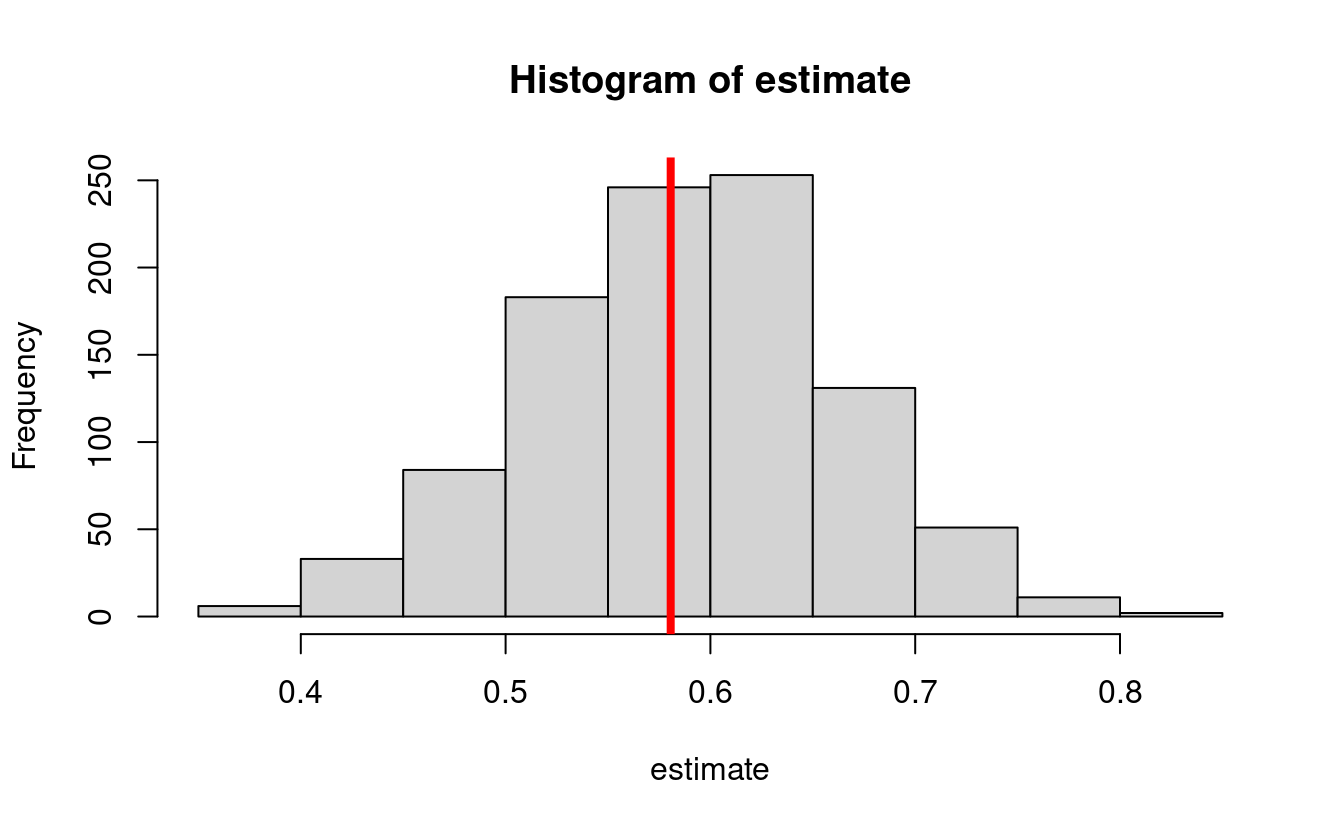
\includegraphics[width=0.8\linewidth]{06-estimation-natural-interventional_files/figure-latex/unnamed-chunk-11-1} \end{center}

\begin{itemize}
\tightlist
\item
  And now the confidence intervals:
\end{itemize}

\begin{lstlisting}[language=R]
cis <- cbind(
  estimate - qnorm(0.975) * sd(estimate),
  estimate + qnorm(0.975) * sd(estimate)
)

ord <- order(rowSums(cis))
lower <- cis[ord, 1]
upper <- cis[ord, 2]
curve(trueval + 0 * x,
  ylim = c(0, 1), xlim = c(0, 1001), lwd = 2, lty = 3, xaxt = "n",
  xlab = "", ylab = "Confidence interval", cex.axis = 1.2, cex.lab = 1.2
)
for (i in 1:1000) {
  clr <- rgb(0.5, 0, 0.75, 0.5)
  if (upper[i] < trueval || lower[i] > trueval) clr <- rgb(1, 0, 0, 1)
  points(rep(i, 2), c(lower[i], upper[i]), type = "l", lty = 1, col = clr)
}
text(450, 0.10, "n=1000 repetitions = 1000 ", cex = 1.2)
text(450, 0.01, paste0(
  "Coverage probability = ",
  mean(lower < trueval & trueval < upper), "%"
), cex = 1.2)
\end{lstlisting}

\begin{center}\includegraphics[width=0.8\linewidth]{06-estimation-natural-interventional_files/figure-latex/unnamed-chunk-12-1} \end{center}

\hypertarget{estimating-indirect-effects-with-r-packages}{%
\chapter{\texorpdfstring{Estimating (in)direct effects with \texttt{R} packages}{Estimating (in)direct effects with R packages}}\label{estimating-indirect-effects-with-r-packages}}

\hypertarget{medshift-stochastic-indirect-effects}{%
\section{\texorpdfstring{\texttt{medshift}: Stochastic (in)direct effects}{medshift: Stochastic (in)direct effects}}\label{medshift-stochastic-indirect-effects}}

We are interested in assessing the population intervention direct effect and
the population intervention indirect effect, based on the effect decomposition
of the population intervention effect introduced in \citet{diaz2020causal}.

To proceed, we'll use as our running example a simple data set from an
observational study of the relationship between BMI and kids behavior,
distributed as part of the \href{https://CRAN.R-project.org/package=mma}{\passthrough{\lstinline!mma!} R package on
CRAN}. First, let's load the packages
we'll be using and set a seed; then, load this data set and take a quick look
at it

\begin{lstlisting}[language=R]
# preliminaries
library(data.table)
library(dplyr)
library(sl3)
library(medshift)
library(mma)
set.seed(429153)

# load and examine data
data(weight_behavior)
dim(weight_behavior)
#> [1] 691  15
head(weight_behavior)
#>      bmi  age sex  race numpeople car gotosch snack tvhours cmpthours cellhours
#> 1 18.207 12.2   F OTHER         5   3       2     1       4         0         0
#> 2 22.784 12.8   M OTHER         4   3       2     1       4         2         0
#> 3 19.607 12.6   F OTHER         4   2       4     2      NA        NA        NA
#> 4 25.568 12.1   M OTHER         2   3       2     1       0         2         0
#> 5 15.074 12.3   M OTHER         4   1       2     1       2         1         3
#> 6 22.983 11.8   M OTHER         4   1       1     1       4         3         2
#>   sports exercises sweat overweigh
#> 1      2         2     1         0
#> 2      1         8     2         0
#> 3   <NA>         4     2         0
#> 4      2         9     1         1
#> 5      1        12     1         0
#> 6      1         1     1         0
\end{lstlisting}

The documentation for the data set describes it as a ``database obtained from the
Louisiana State University Health Sciences Center, New Orleans, by Dr.~Richard
Scribner. He explored the relationship between BMI and kids behavior through a
survey at children, teachers and parents in Grenada in 2014. This data set
includes 691 observations and 15 variables.''

Unfortunately, the data set contains a few observations with missing values. As
these are unrelated to the object of our analysis, we'll simply remove these for
the time being. Note that in a real data analysis, we might consider strategies
to fully make of the observed data, perhaps by imputing missing values. For now,
we simply remove the incomplete observations, resulting in a data set with fewer
observations but much the same structure as the original:

\begin{lstlisting}[language=R]
# remove missing values
is_na <- unique(do.call(c, apply(apply(weight_behavior, 2, is.na), 2, which)))
weight_behavior_complete <- weight_behavior[-is_na, ]
weight_behavior_complete$sports <-
  as.numeric(weight_behavior_complete$sports) - 1
dim(weight_behavior_complete)
#> [1] 567  15
head(weight_behavior_complete)
#>      bmi  age sex  race numpeople car gotosch snack tvhours cmpthours cellhours
#> 1 18.207 12.2   F OTHER         5   3       2     1       4         0         0
#> 2 22.784 12.8   M OTHER         4   3       2     1       4         2         0
#> 4 25.568 12.1   M OTHER         2   3       2     1       0         2         0
#> 5 15.074 12.3   M OTHER         4   1       2     1       2         1         3
#> 6 22.983 11.8   M OTHER         4   1       1     1       4         3         2
#> 8 19.157 12.1   F OTHER         3   3       2     1       0         0         1
#>   sports exercises sweat overweigh
#> 1      1         2     1         0
#> 2      0         8     2         0
#> 4      1         9     1         1
#> 5      0        12     1         0
#> 6      0         1     1         0
#> 8      0         1     3         0
\end{lstlisting}

For the analysis of this observational data set, we focus on the effect of
participating in a sports team (\passthrough{\lstinline!sports!}) on the BMI of children (\passthrough{\lstinline!bmi!}), taking
several related covariates as mediators (\passthrough{\lstinline!snack!}, \passthrough{\lstinline!exercises!}, \passthrough{\lstinline!overweigh!}) and
all other collected covariates as potential confounders. Considering an NPSEM,
we separate the observed variables from the data set into their corresponding
nodes as follows

\begin{lstlisting}[language=R]
Y <- weight_behavior_complete$bmi
A <- weight_behavior_complete$sports
Z <- weight_behavior_complete %>%
  select(snack, exercises, overweigh)
W <- weight_behavior_complete %>%
  select(
    age, sex, race, numpeople, car, gotosch, tvhours, cmpthours,
    cellhours, sweat
  )
\end{lstlisting}

Finally, in our analysis, we consider an incremental propensity score
intervention (IPSI), as first proposed by \citet{kennedy2017nonparametric}, wherein the
\emph{odds of participating in a sports team} is modulated by some fixed amount
(\(0 \leq \delta \leq \infty\)) for each individual. Such an intervention may be
interpreted as the effect of a school program that motivates children to
participate in sports teams. To exemplify our approach, we postulate a
motivational intervention that \emph{triples the odds} of participating in a sports
team for each individual:

\begin{lstlisting}[language=R]
delta_shift_ipsi <- 3
\end{lstlisting}

To easily incorporate ensemble machine learning into the estimation procedure,
we rely on the facilities provided in the \href{https://tlverse.org/sl3}{\passthrough{\lstinline!sl3!} R
package} \citep{coyle2020sl3}. For a complete guide on using
the \passthrough{\lstinline!sl3!} R package, consider consulting \url{https://tlverse.org/sl3}, or
\url{https://tlverse.org} (and \url{https://github.com/tlverse}) for the \passthrough{\lstinline!tlverse!}
ecosystem, of which \passthrough{\lstinline!sl3!} is a major part. We construct an ensemble learner
using a handful of popular machine learning algorithms below

\begin{lstlisting}[language=R]
# SL learners used for continuous data (the nuisance parameter M)
xgb_contin_lrnr <- Lrnr_xgboost$new(nrounds = 50, objective = "reg:linear")
enet_contin_lrnr <- Lrnr_glmnet$new(
  alpha = 0.5, family = "gaussian",
  nfolds = 3
)
lasso_contin_lrnr <- Lrnr_glmnet$new(
  alpha = 1, family = "gaussian",
  nfolds = 3
)
fglm_contin_lrnr <- Lrnr_glm_fast$new(family = gaussian())
contin_lrnr_lib <- Stack$new(
  enet_contin_lrnr, lasso_contin_lrnr,
  fglm_contin_lrnr, xgb_contin_lrnr
)
sl_contin_lrnr <- Lrnr_sl$new(
  learners = contin_lrnr_lib,
  metalearner = Lrnr_nnls$new()
)

# SL learners used for binary data (nuisance parameters G and E in this case)
xgb_binary_lrnr <- Lrnr_xgboost$new(nrounds = 50, objective = "reg:logistic")
enet_binary_lrnr <- Lrnr_glmnet$new(
  alpha = 0.5, family = "binomial",
  nfolds = 3
)
lasso_binary_lrnr <- Lrnr_glmnet$new(
  alpha = 1, family = "binomial",
  nfolds = 3
)
fglm_binary_lrnr <- Lrnr_glm_fast$new(family = binomial())
binary_lrnr_lib <- Stack$new(
  enet_binary_lrnr, lasso_binary_lrnr,
  fglm_binary_lrnr, xgb_binary_lrnr
)
logistic_metalearner <- make_learner(
  Lrnr_solnp,
  metalearner_logistic_binomial,
  loss_loglik_binomial
)
sl_binary_lrnr <- Lrnr_sl$new(
  learners = binary_lrnr_lib,
  metalearner = logistic_metalearner
)
\end{lstlisting}

\hypertarget{decomposing-the-population-intervention-effect}{%
\subsection{Decomposing the population intervention effect}\label{decomposing-the-population-intervention-effect}}

We may decompose the population intervention effect (PIE) in terms of a
\emph{population intervention direct effect} (PIDE) and a \emph{population
intervention indirect effect} (PIIE):
\begin{equation*}
  \overbrace{\mathbb{E}\{Y(A_\delta, Z(A_\delta)) -
    Y(A_\delta, Z)\}}^{\text{PIIE}} +
    \overbrace{\mathbb{E}\{Y(A_\delta, Z) - Y(A, Z)\}}^{\text{PIDE}}.
\end{equation*}

This decomposition of the PIE as the sum of the population intervention direct
and indirect effects has an interpretation analogous to the corresponding
standard decomposition of the average treatment effect. In the sequel, we will
compute each of the components of the direct and indirect effects above using
appropriate estimators as follows

\begin{itemize}
\tightlist
\item
  For \(\mathbb{E}\{Y(A, Z)\}\), the sample mean \(\frac{1}{n}\sum_{i=1}^n Y_i\) is
  sufficient;
\item
  for \(\mathbb{E}\{Y(A_{\delta}, Z)\}\), an efficient one-step estimator for the
  effect of a joint intervention altering the exposure mechanism but not the
  mediation mechanism, as proposed in \citet{diaz2020causal}; and,
\item
  for \(\mathbb{E}\{Y(A_{\delta}, Z_{A_{\delta}})\}\), an efficient one-step
  estimator for the effect of a joint intervention altering both the exposure
  and mediation mechanisms, as proposed in \citet{kennedy2017nonparametric} and
  implemented in the \href{https://github.com/ehkennedy/npcausal}{\passthrough{\lstinline!npcausal!} R
  package}.
\end{itemize}

\hypertarget{estimating-the-effect-decomposition-term}{%
\subsection{Estimating the effect decomposition term}\label{estimating-the-effect-decomposition-term}}

As given in \citet{diaz2020causal}, the statistical functional identifying the
decomposition term that appears in both the PIDE and PIIE
\(\mathbb{E}\{Y(A_{\delta}, Z)\}\), which corresponds to altering the exposure
mechanism while keeping the mediation mechanism fixed, is
\begin{equation*}
  \theta_0(\delta) = \int m_0(a, z, w) g_{0,\delta}(a \mid w) p_0(z, w)
    d\nu(a, z, w),
\end{equation*}
for which a one-step estimator is available. The corresponding \emph{efficient
influence function} (EIF) with respect to the nonparametric model \(\mathcal{M}\)
is \(D_{\eta,\delta}(o) = D^Y_{\eta,\delta}(o) + D^A_{\eta,\delta}(o) + D^{Z,W}_{\eta,\delta}(o) - \theta(\delta)\). The
one-step estimator may be computed using the EIF estimating equation, making use
of cross-fitting \citep{zheng2011cross, chernozhukov2018double} to circumvent any
need for entropy conditions (i.e., Donsker class restrictions). The resultant
estimator is
\begin{equation*}
  \hat{\theta}(\delta) = \frac{1}{n} \sum_{i = 1}^n D_{\hat{\eta}_{j(i)},
  \delta}(O_i) = \frac{1}{n} \sum_{i = 1}^n \left\{ D^Y_{\hat{\eta}_{j(i)},
  \delta}(O_i) + D^A_{\hat{\eta}_{j(i)}, \delta}(O_i) +
  D^{Z,W}_{\hat{\eta}_{j(i)}, \delta}(O_i) \right\},
\end{equation*}
which is implemented in the \passthrough{\lstinline!medshift!} R package. We make use of that
implementation to estimate \(\mathbb{E}\{Y(A_{\delta}, Z)\}\) via its one-step
estimator \(\hat{\theta}(\delta)\) below

\begin{lstlisting}[language=R]
# let's compute the parameter where A (but not Z) are shifted
theta_eff <- medshift(
  W = W, A = A, Z = Z, Y = Y,
  delta = delta_shift_ipsi,
  g_learners = sl_binary_lrnr,
  e_learners = sl_binary_lrnr,
  m_learners = sl_contin_lrnr,
  phi_learners = Lrnr_hal9001$new(),
  estimator = "onestep",
  estimator_args = list(cv_folds = 3)
)
summary(theta_eff)
\end{lstlisting}

\hypertarget{estimating-the-direct-effect}{%
\subsection{Estimating the direct effect}\label{estimating-the-direct-effect}}

Recall that, based on the decomposition outlined previously, the population
intervention direct effect may be denoted \(\beta_{\text{PIDE}}(\delta) = \theta_0(\delta) - \mathbb{E}Y\). Thus, an estimator of the PIDE,
\(\hat{\beta}_{\text{PIDE}}(\delta)\) may be expressed as a composition of
estimators of its constituent parameters:
\begin{equation*}
  \hat{\beta}_{\text{PIDE}}({\delta}) = \hat{\theta}(\delta) -
  \frac{1}{n} \sum_{i = 1}^n Y_i.
\end{equation*}

Based on the above, we may construct an estimator of the PIDE using quantities
already computed. The convenience function below applies the simple delta method
required in the case of a linear contrast between the two constituent
parameters:

\begin{lstlisting}[language=R]
# convenience function to compute inference via delta method: EY1 - EY0
linear_contrast <- function(params, eifs, ci_level = 0.95) {
  # bounds for confidence interval
  ci_norm_bounds <- c(-1, 1) * abs(stats::qnorm(p = (1 - ci_level) / 2))
  param_est <- params[[1]] - params[[2]]
  eif <- eifs[[1]] - eifs[[2]]
  se_eif <- sqrt(var(eif) / length(eif))
  param_ci <- param_est + ci_norm_bounds * se_eif
  # parameter and inference
  out <- c(param_ci[1], param_est, param_ci[2])
  names(out) <- c("lwr_ci", "param_est", "upr_ci")
  return(out)
}
\end{lstlisting}

With the above convenience function in hand, we'll construct or extract the
necessary components from existing objects and simply apply the function:

\begin{lstlisting}[language=R]
# parameter estimates and EIFs for components of direct effect
EY <- mean(Y)
eif_EY <- Y - EY
params_de <- list(theta_eff$theta, EY)
eifs_de <- list(theta_eff$eif, eif_EY)

# direct effect = EY - estimated quantity
de_est <- linear_contrast(params_de, eifs_de)
de_est
\end{lstlisting}

\hypertarget{medoutcon-naturalinterventional-effects}{%
\section{\texorpdfstring{\texttt{medoutcon}: Natural/Interventional Effects}{medoutcon: Natural/Interventional Effects}}\label{medoutcon-naturalinterventional-effects}}

An exposure of interest often affects an outcome directly, or indirectly by the
mediation of some intermediate variables. Identifying and quantifying the
mechanisms underlying causal effects is an increasingly popular endeavor in
public health, medicine, and the social sciences, as knowledge of such
mechanisms can improve understanding of both \emph{why and how} treatments can be
effective. Such mechanistic knowledge may be arguably even more important in
cases where treatments result in unanticipated ineffective or even harmful
effects.

Traditional techniques for mediation analysis fare poorly in the face of
intermediate confounding. Classical parameters like the natural (in)direct
effects face a lack of identifiability in cases where mediator-outcome (i.e.,
intermediate) confounders affected by exposure complicate the relationship
between the exposure, mediators, and outcome. \citet{diaz2020nonparametric} provide a
theoretical and computational study of the properties of newly developed
interventional (in)direct effect estimands within the non-parametric statistical
model. Among their contributions, \citet{diaz2020nonparametric}

\begin{itemize}
\tightlist
\item
  derive the efficient influence function (EIF), an key object in
  semiparametric efficiency theory;
\item
  use the EIF to develop two asymptotically optimal, non-parametric estimators,
  each of which is capable of leveraging machine learning for the estimation of
  nuisance parameters; and
\item
  present theoretical conditions under which their proposed estimators are
  consistent, multiply robust, and efficient.
\end{itemize}

\hypertarget{problem-setup-and-notation}{%
\subsection{Problem Setup and Notation}\label{problem-setup-and-notation}}

The problem addressed by the work of \citet{diaz2020nonparametric} may be represented
by the following nonparametric structural equation model (NPSEM):
\begin{align*}
  W &= f_W(U_W); A = f_A(W, U_A); Z=f_Z(W, A, U_Z);\\ \nonumber
  M &= f_M(W, A, Z, U_M); Y = f_Y(W, A, Z, M, U_Y).
\end{align*}
In the NPSEM, \(W\) denotes a vector of observed pre-treatment covariates, \(A\)
denotes a categorical treatment variable, \(Z\) denotes an intermediate confounder
affected by treatment, \(M\) denotes a (possibly multivariate) mediator, and \(Y\)
denotes a continuous or binary outcome. The vector of exogenous factors
\(U=(U_W,U_A,U_Z,U_M,U_Y)\), and the functions \(f\), are assumed deterministic but
unknown. Importantly, the NPSEM encodes a time-ordering between these variables
and allows the evaluation of counterfactual quantities defined by intervening on
a set of nodes of the NPSEM. The observed data unit can be represented by the
random variable \(O = (W, A, Z, M, Y)\); we consider access to \(O_1, \ldots, O_n\),
a sample of \(n\) i.i.d. observations of \(O\).

\citet{diaz2020nonparametric} additionally define the following parameterizations,
familiarity with which will be useful for using the \href{https://github.com/nhejazi/medoutcon}{\passthrough{\lstinline!medoutcon!} \passthrough{\lstinline!R!}
package}. In particular, these authors
define \(g(a \mid w)\) as the probability mass function of \(A = a\) conditional on
\(W = w\) and use \(h(a \mid m, w)\) to denote the probability mass function of \(A = a\) conditional on \((M, W) = (m, w)\). Further, \citet{diaz2020nonparametric} use
\(b(a, z, m, w)\) to denote the outcome regression function \(\mathbb{E}(Y \mid A = a, Z = z, M = m, W = w)\), as well as \(q(z \mid a,w)\) and \(r(z \mid a, m, w)\)
to denote the corresponding conditional densities of \(Z\).

\hypertarget{interventional-indirect-effects-1}{%
\subsection{Interventional (In)Direct Effects}\label{interventional-indirect-effects-1}}

\citet{diaz2020nonparametric} define the \emph{total effect} of \(A\) on \(Y\) in terms of a
contrast between two user-supplied values \(a', a^{\star} \in \mathcal{A}\).
Examination of the NPSEM reveals that there are four paths involved in this
effect, namely \(A \rightarrow Y\), \(A \rightarrow M \rightarrow Y\), \(A \rightarrow Z \rightarrow Y\), and \(A \rightarrow Z \rightarrow M \rightarrow Y\).
Mediation analysis has classically considered the \emph{natural direct effect} (NDE)
and the \emph{natural indirect effect} (NIE), which are defined as
\(\mathbb{E}_c(Y_{a', M_{a^{\star}}} - Y_{a^{\star}, M_{a^{\star}}})\) and
\(\mathbb{E}_c(Y_{a',M_{a'}} - Y_{a',M_{a^{\star}}})\), respectively. The natural
direct effect measures the effect through paths \emph{not} involving the mediator
(\(A \rightarrow Y\) and \(A \rightarrow Z \rightarrow Y\)), whereas the natural
indirect effect measures the effect through paths involving the mediator
(\(A \rightarrow M \rightarrow Y\) and \(A \rightarrow Z \rightarrow M \rightarrow Y\)). As the sum of the natural direct and indirect effects equals the average
treatment effect \(\mathbb{E}_c(Y_1-Y_0)\), this effect decomposition is
appealing. Unfortunately, the natural direct and indirect effects are
not generally identified in the presence of an intermediate confounder affected
by treatment.

To circumvent this issue, \citet{diaz2020nonparametric} define the direct and indirect
effects using stochastic interventions on the mediator, following a strategy
previously outlined by \citet{vanderweele2014effect} and \citet{rudolph2017robust}, among
others. Let \(G_a\) denote a random draw from the conditional distribution of
\(M_a\) conditional on \(W\). Consider the effect of \(A\) on \(Y\) defined as the
difference in expected outcome in hypothetical worlds in which \((A,M) = (a', G_{a'})\) versus \((A,M) = (a^{\star}, G_{a^{\star}})\) with probability one, which
may be decomposed into direct and indirect effects as follows
\begin{equation*}
\mathbb{E}_c(Y_{a', G_{a'}} - Y_{a^{\star}, G_{a^{\star}}}) =
  \underbrace{\mathbb{E}_c(Y_{a', G_{a'}} - Y_{a',
    G_{a^{\star}}})}_{\text{Indirect effect (through $M$)}} +
  \underbrace{\mathbb{E}_c(Y_{a', G_{a^{\star}}} - Y_{a^{\star},
      G_{a^{\star}}})}_{\text{Direct effect (not through $M$)}}.
\end{equation*}
Like the natural direct effect, this interventional direct effect measures the
effects through paths not involving the mediator. Likewise, the interventional
indirect effect measures the effect through paths involving the mediator. Note,
however, that natural and interventional mediation effects have different
interpretations. That is, the interventional indirect effect measures the effect
of fixing the exposure at \(a'\) while setting the mediator to a random draw
\(G_{a^{\star}}\) from those with exposure \(a'\) versus a random draw \(G_{a'}\) from
those with exposure \(a^{\star}\), given covariates \(W\). As is clear from the
effect decomposition, the term \(\theta_c = \mathbb{E}_c(Y_{a', G_{a^{\star}}})\)
is required for estimation of both the interventional direct and indirect
effects; thus, \citet{diaz2020nonparametric} focus on estimation of this quantity.
Importantly, it has been shown that \(\theta_c\) is identified by the statistical
functional
\begin{equation*}
  \theta = \int b(a', z, m, w) q(z \mid a', w) p(m \mid a^{\star}, w)
    p(w) d\nu(w,z,m)
\end{equation*}
under a set of standard identifiability conditions \citep{vanderweele2014effect},
which are further reviewed in \citet{diaz2020nonparametric}.

\hypertarget{efficient-estimation}{%
\subsection{Efficient Estimation}\label{efficient-estimation}}

\citet{diaz2020nonparametric} define two efficient estimators of their interventional
(in)direct effects. These are based on the one-step estimation and targeted
minimum loss (TML) estimation frameworks, respectively. Briefly, both estimation
strategies proceed in two stages, starting by first constructing initial
estimates of the nuisance parameters present in the EIF, then proceeding to
apply distinct bias-correction strategies in their second stages. Both
estimation strategies require an assumption about the behavior of initial
estimators of the nuisance parameters (specifically, that these lie in a Donsker
class); however, the need for such an assumption may be avoided by making use of
cross-validation in the fitting fo initial estimators. The \passthrough{\lstinline!medoutcon!} \passthrough{\lstinline!R!}
package requires the use of cross-validation in the construction of these
initial estimates, resulting in cross-fitted one-step and and cross-validated
TML estimators \citep{klaassen1987consistent, zheng2011cross, chernozhukov2018double}.

The one-step estimator \(\hat{\theta}_{\text{os}}\) is constructed by adding the
empirical mean of the EIF (evaluated at initial estimates of the nuisance
parameters) to the substitution estimator. By constrast, the TML estimator
\(\hat{\theta}_{\text{tmle}}\) updates the components of the substitution
estimator via logistic tilting models formulated to ensure that relevant score
equations appearing in the EIF are (approximately) solved. While the estimators
are asymptotically equivalent, TML estimators have been shown to exhibit
superior finite-sample performance, making them potentially more reliable than
one-step estimators. For the exact form of the EIF as well as those of the
one-step and TML estimators, consult \citet{diaz2020nonparametric}.

\hypertarget{data-analysis-example}{%
\subsection{Data Analysis Example}\label{data-analysis-example}}

\hypertarget{setting-up-the-data-example}{%
\subsubsection{Setting up the data example}\label{setting-up-the-data-example}}

Now, we'll take a look at how to estimate the interventional direct and indirect
effects using a simulated data example. \citet{diaz2020nonparametric} illustrate the
use of their estimators of these effects in an application in which they seek to
elucidate the mechanisms behind the unintended harmful effects that a housing
intervention had on adolescent girls' risk behavior.

First, let's load a few required packages and set a seed for our simulation.

\begin{lstlisting}[language=R]
library(data.table)
library(medoutcon)
library(sl3)
set.seed(75681)
n_obs <- 500
\end{lstlisting}

Next, we'll generate a very simple simulated dataset. The function
\passthrough{\lstinline!make\_example\_data!}, defined below, generates three binary baseline covariates
\(W = (W_1, W_2, W_3)\), a binary exposure variable \(A\), a single binary mediateor
\(M\) an intermediate confounder \(Z\) that affects the mediator \(M\) and is itself
affected by the exposure \(A\), and, finally, a binary outcome \(Y\) that is a
function of \((W, A, Z, M)\).

\begin{lstlisting}[language=R]
# produces a simple data set based on ca causal model with mediation
make_example_data <- function(n_obs = 1000) {
  ## baseline covariates
  w_1 <- rbinom(n_obs, 1, prob = 0.6)
  w_2 <- rbinom(n_obs, 1, prob = 0.3)
  w_3 <- rbinom(n_obs, 1, prob = pmin(0.2 + (w_1 + w_2) / 3, 1))
  w <- cbind(w_1, w_2, w_3)
  w_names <- paste("W", seq_len(ncol(w)), sep = "_")

  ## exposure
  a <- as.numeric(rbinom(n_obs, 1, plogis(rowSums(w) - 2)))

  ## mediator-outcome confounder affected by treatment
  z <- rbinom(n_obs, 1, plogis(rowMeans(-log(2) + w - a) + 0.2))

  ## mediator -- could be multivariate
  m <- rbinom(n_obs, 1, plogis(rowSums(log(3) * w[, -3] + a - z)))
  m_names <- "M"

  ## outcome
  y <- rbinom(n_obs, 1, plogis(1 / (rowSums(w) - z + a + m)))

  ## construct output
  dat <- as.data.table(cbind(w = w, a = a, z = z, m = m, y = y))
  setnames(dat, c(w_names, "A", "Z", m_names, "Y"))
  return(dat)
}

# set seed and simulate example data
example_data <- make_example_data(n_obs)
w_names <- stringr::str_subset(colnames(example_data), "W")
m_names <- stringr::str_subset(colnames(example_data), "M")
\end{lstlisting}

Now, let's take a quick look at our simulated data:

\begin{lstlisting}[language=R]
# quick look at the data
head(example_data)
#>    W_1 W_2 W_3 A Z M Y
#> 1:   0   0   1 0 0 0 1
#> 2:   0   1   1 0 0 0 1
#> 3:   1   1   0 0 1 1 1
#> 4:   1   0   1 0 1 0 0
#> 5:   0   0   0 1 1 1 1
#> 6:   1   0   1 1 0 1 1
\end{lstlisting}

As noted above, all covariates in our dataset are binary; however, note that
this need not be the case for using our methodology --- in particular, the only
current limitation is that the intermediate confounder \(Z\) must be binary when
using our implemented TML estimator of the (in)direct effects.

Using this dataset, we'll proceed to estimate the interventional (in)direct
effects. In order to do so, we'll need to estimate several nuisance parameters,
including the exposure mechanism \(g(A \mid W)\), a re-parameterized exposure
mechanism that conditions on the mediators \(h(A \mid M, W)\), the outcome
mechanism \(b(Y \mid M, Z, A, W)\), and two variants of the intermediate
confounding mechanism \(q(Z \mid A, W)\) and \(r(Z \mid M, A, W)\). In order to
estimate each of these nuisance parameters flexibly, we'll rely on data adaptive
regression strategies in order to avoid the potential for (parametric) model
misspecification.

\hypertarget{ensemble-learning-of-nuisance-functions}{%
\subsubsection{Ensemble learning of nuisance functions}\label{ensemble-learning-of-nuisance-functions}}

As we'd like to rely on flexible, data adaptive regression strategies for
estimating each of the nuisance parameters \((g, h, b, q, r)\), we require a
method for choosing among or combining the wide variety of available regression
strategies. For this, we recommend the use of the Super Learner algorithm for
ensemble machine learning \citep{vdl2007super}. The recently developed \href{https://tlverse.org/sl3}{\passthrough{\lstinline!sl3!} R
package} \citep{coyle2020sl3} provides a unified interface
for deploying a wide variety of machine learning algorithms (simply called
\emph{learners} in the \passthrough{\lstinline!sl3!} nomenclature) as well as for constructing Super Learner
ensemble models of such learners. For a complete guide on using the \passthrough{\lstinline!sl3!} R
package, consider consulting \url{https://tlverse.org/sl3}, or \url{https://tlverse.org}
(and \url{https://github.com/tlverse}) for the \passthrough{\lstinline!tlverse!} ecosystem, of which \passthrough{\lstinline!sl3!} is
an integral part.

To construct an ensemble learner using a handful of popular machine learning
algorithms, we'll first instantiate variants of learners from the appropriate
classes for each algorithm, and then create a Super Learner ensemble via the
\passthrough{\lstinline!Lrnr\_sl!} class. Below, we demonstrate the construction of an ensemble learner
based on a modeling library including an intercept model, a main-terms GLM,
\(\ell_1\)-penalized Lasso regression, an elastic net regression that equally
weights the \(\ell_1\) and \(\ell_2\) penalties, random forests (\passthrough{\lstinline!ranger!}), and the
highly adaptive lasso (HAL):

\begin{lstlisting}[language=R]
# instantiate learners
mean_lrnr <- Lrnr_mean$new()
fglm_lrnr <- Lrnr_glm_fast$new(family = binomial())
lasso_lrnr <- Lrnr_glmnet$new(alpha = 1, family = "binomial", nfolds = 3)
enet_lrnr <- Lrnr_glmnet$new(alpha = 0.5, family = "binomial", nfolds = 3)
rf_lrnr <- Lrnr_ranger$new(num.trees = 200)

# for HAL, use linear probability formulation, with bounding in unit interval
hal_gaussian_lrnr <- Lrnr_hal9001$new(
  family = "gaussian",
  fit_control = list(
    max_degree = 3,
    n_folds = 3,
    use_min = TRUE,
    type.measure = "mse"
  )
)
bound_lrnr <- Lrnr_bound$new(bound = 1e-6)
hal_bounded_lrnr <- Pipeline$new(hal_gaussian_lrnr, bound_lrnr)

# create learner library and instantiate super learner ensemble
lrnr_lib <- Stack$new(
  mean_lrnr, fglm_lrnr, enet_lrnr, lasso_lrnr,
  rf_lrnr, hal_bounded_lrnr
)
sl_lrnr <- Lrnr_sl$new(learners = lrnr_lib, metalearner = Lrnr_nnls$new())
\end{lstlisting}

While we recommend the use of a Super Learner ensemble model like the one
constructed above in practice, such a library will be too computationally
intensive for our examples. To reduce computation time, we construct a simpler
library, using only a subset of the above learning algorithms:

\begin{lstlisting}[language=R]
# create simpler learner library and instantiate super learner ensemble
lrnr_lib <- Stack$new(mean_lrnr, fglm_lrnr, lasso_lrnr, rf_lrnr)
sl_lrnr <- Lrnr_sl$new(learners = lrnr_lib, metalearner = Lrnr_nnls$new())
\end{lstlisting}

Having set up our ensemble learner, we're now ready to estimate each of the
interventional effects using the efficient estimators exposed in the \passthrough{\lstinline!medoutcon!}
package.

\hypertarget{estimating-the-direct-effect-1}{%
\subsubsection{Estimating the direct effect}\label{estimating-the-direct-effect-1}}

We're now ready to estimate the interventional direct effect. This direct effect
is computed as a contrast between the interventions \((a' = 1, a^{\star} = 0)\)
and \((a' = 0, a^{\star} = 0)\). In particular, our efficient estimators of the
interventional direct effect proceed by constructing estimators
\(\hat{\theta}(a' = 1, a^{\star} = 0)\) and \(\hat{\theta}(a' = 0, a^{\star} = 0)\).
Then, an efficient estimator of the direct effect is available by application
of the delta method, that is, \(\hat{\theta}^{\text{DE}} = \hat{\theta}(a' = 1, a^{\star} = 0) - \hat{\theta}(a' = 0, a^{\star} = 0)\).
Applying the same principle to the EIF estimates, one can derive variance
estimates and construct asymptotically correct Wald-style confidence intervals
for \(\hat{\theta}^{\text{DE}}\).

The \passthrough{\lstinline!medoutcon!} package makes the estimation task quite simple, as only a single
call to the eponymous \passthrough{\lstinline!medoutcon!} function is required. As demonstrated below,
we need only feed in each component of the observed data \(O = (W, A, Z, M, Y)\)
(of which \(W\) and \(M\) can be multivariate), specify the effect type, and the
estimator. Additionally, for each nuisance parameter we may specify a separate
regression function --- in the examples below, we use the simpler Super Learner
ensemble constructed above for fitting each nuisance function, but this need not
be the case (i.e., different estimators may be used for each nuisance function).

First, we examine the one-step estimator of the interventional direct effect.
Recall that the one-step estimator is constructed by adding the mean of the EIF
(evaluated at initial estimates of the nuisance parameters) to the substitution
estimator. As noted above, this is done separately for each of the two contrasts
\((a' = 0, a^{\star} = 0)\) and \((a' = 1, a^{\star} = 0)\). Thus, the one-step
estimator of this direct effect is constructed by application of the delta
method to each of the one-step estimators (and EIFs) for these contrasts.

\begin{lstlisting}[language=R]
# compute one-step estimate of the interventional direct effect
os_de <- medoutcon(
  W = example_data[, ..w_names],
  A = example_data$A,
  Z = example_data$Z,
  M = example_data[, ..m_names],
  Y = example_data$Y,
  g_learners = sl_lrnr,
  h_learners = sl_lrnr,
  b_learners = sl_lrnr,
  q_learners = sl_lrnr,
  r_learners = sl_lrnr,
  effect = "direct",
  estimator = "onestep",
  estimator_args = list(cv_folds = 2)
)
summary(os_de)
\end{lstlisting}

Next, let's compare the one-step estimate to the TML estimate. Analogous to the
case of the one-step estimator, the TML estimator can be evaluated via a single
call to the \passthrough{\lstinline!medoutcon!} function:

\begin{lstlisting}[language=R]
# compute targeted minimum loss estimate of the interventional direct effect
tmle_de <- medoutcon(
  W = example_data[, ..w_names],
  A = example_data$A,
  Z = example_data$Z,
  M = example_data[, ..m_names],
  Y = example_data$Y,
  g_learners = sl_lrnr,
  h_learners = sl_lrnr,
  b_learners = sl_lrnr,
  q_learners = sl_lrnr,
  r_learners = sl_lrnr,
  effect = "direct",
  estimator = "tmle",
  estimator_args = list(cv_folds = 2, max_iter = 5)
)
summary(tmle_de)
\end{lstlisting}

Here, we recall that the TML estimator generally exhibits better finite-sample
performance than the one-step estimator \citep{vdl2011targeted, vdl2018targeted}, so
the TML estimate is likely to be more reliable in modest (realistic) sample
sizes.

\hypertarget{estimating-the-indirect-effect}{%
\subsubsection{Estimating the indirect effect}\label{estimating-the-indirect-effect}}

Estimation of the interventional indirect effect proceeds similarly to the
strategy discussed above for the corresponding direct effect. An efficient
estimator can be computed as a contrast between the interventions \((a' = 1, a^{\star} = 0)\) and \((a' = 1, a^{\star} = 1)\). Specifically, our efficient
estimators of the interventional indirect effect proceed by constructing
estimators \(\hat{\theta}(a' = 1, a^{\star} = 0)\) and \(\hat{\theta}(a' = 1, a^{\star} = 1)\). Then, application of the delta method yields an efficient
estimator of the indirect effect, that is, \(\hat{\theta}^{\text{IE}} = \hat{\theta}(a' = 1, a^{\star} = 0) - \hat{\theta}(a' = 1, a^{\star} = 1)\). The
same principle may be applied to the EIF estimates to derive variance estimates
and construct asymptotically correct Wald-style confidence intervals for
\(\hat{\theta}^{\text{IE}}\).

Now, we examine the one-step estimator of the interventional indirect effect.
The one-step estimator is constructed by adding the mean of the EIF
(evaluated at initial estimates of the nuisance parameters) to the substitution
estimator. As noted above, this is done separately for each of the two contrasts
\((a' = 1, a^{\star} = 1)\) and \((a' = 1, a^{\star} = 0)\). Thus, the one-step
estimator of this indirect effect is constructed by application of the delta
method to each of the one-step estimators (and EIFs) for the contrasts.

\begin{lstlisting}[language=R]
# compute one-step estimate of the interventional indirect effect
os_ie <- medoutcon(
  W = example_data[, ..w_names],
  A = example_data$A,
  Z = example_data$Z,
  M = example_data[, ..m_names],
  Y = example_data$Y,
  g_learners = sl_lrnr,
  h_learners = sl_lrnr,
  b_learners = sl_lrnr,
  q_learners = sl_lrnr,
  r_learners = sl_lrnr,
  effect = "indirect",
  estimator = "onestep"
)
summary(os_ie)
\end{lstlisting}

As before, let's compare the one-step estimate to the TML estimate. Analogous
to the case of the one-step estimator, the TML estimator can be evaluated via a
single call to the \passthrough{\lstinline!medoutcon!} function, as demonstrated below

\begin{lstlisting}[language=R]
# compute targeted minimum loss estimate of the interventional indirect effect
tmle_ie <- medoutcon(
  W = example_data[, ..w_names],
  A = example_data$A,
  Z = example_data$Z,
  M = example_data[, ..m_names],
  Y = example_data$Y,
  g_learners = sl_lrnr,
  h_learners = sl_lrnr,
  b_learners = sl_lrnr,
  q_learners = sl_lrnr,
  r_learners = sl_lrnr,
  effect = "indirect",
  estimator = "tmle"
)
summary(tmle_ie)
\end{lstlisting}

As before, the TML estimator provides better finite-sample performance than the
one-step estimator, so it may be preferred in this example.

  \bibliography{book.bib,packages.bib}

\backmatter
\printindex

\end{document}
